\documentclass[letterpaper,10pt]{article}
\usepackage{soul}
\usepackage{graphicx,xcolor}
\usepackage{amsmath,amsthm}
\usepackage{amssymb}
\usepackage{float}
\usepackage[hidelinks]{hyperref}
\usepackage{enumerate}
\usepackage{mathrsfs}
\usepackage{mathtools}

\usepackage[english]{babel}

\theoremstyle{plain}

\newtheorem*{theorem*}{Theorem}
\newtheorem{theorem}{Theorem}[section]
\newtheorem{claim}{Claim}[section]
\newtheorem{definition}{Definition}[section]
\newtheorem{lemma}[theorem]{Lemma}
\newtheorem{proposition}[theorem]{Proposition}
\newtheorem{corollary}[theorem]{Corollary}
\newtheorem{conjecture}[theorem]{Conjecture}
\newtheorem*{question*}{Question}
\newtheorem*{questions*}{Questions}
\newtheorem*{remark*}{Remark}
\newtheorem*{example*}{Example}

\newcommand{\BS}[1][N]{\mathrm{BS}(1,#1)}
\def\htop{h_{\mathrm{top}}}
%\def\NN{\mathbb{N}}
%\def\ZZ{\mathbb{Z}}
%\def\RR{\mathbb{R}}
%\def\prob{\mathbb{P}}
%\def\esp{\mathbb{E}}
%\def\ag{\mathcal{A}}
%\def\bg{\mathcal{B}}
%\def\CC{\mathcal{C}}
%\def\cg{\mathcal{C}}
%\def\FF{\mathcal{F}}
%\def\dens{\operatorname{dens}}

\newcommand{\define}[1]{\emph{#1}}
\newcommand{\cor}[2][]{#2}

%TIKZ
\usepackage{tikz}
\usetikzlibrary{patterns,positioning,arrows,decorations.markings,calc,decorations.pathmorphing,decorations.pathreplacing}
\usepackage{tikz-qtree}
\RequirePackage{pgffor} % foreach
%\usetikzlibrary{lindenmayersystems}
%\usetikzlibrary{arrows}
%\usepackage{tikz-3dplot}

%\pgfdeclarelindenmayersystem{cayleyPSL2Z}{
%	\rule{A -> [FB+FF[+A]----FF[+A]----FF]++++++}
%	\rule{B -> FBB}}

% %Colors :
% 
%\definecolor{vert}{RGB}{0,178,102}


\title{Periodicity constraints and graph-coloring subshifts on ascending HNN-extensions of an abelian group}
\date{\today}
\author{Eduardo Silva \\
	\texttt{esilva@dim.uchile.cl}}



\begin{document}
	
	\maketitle 
	
	\begin{abstract}
	abstract
	\end{abstract}	
	
	%\textbf{Keywords:} Symbolic, Keyword 2, Keyword 3.
	
	%%%%%%%%%%%%%%%%%%%%%%
	%%%%%%%%%%%%%%%%%%%%%%
	\section*{Introduction}
	\label{section.introduction}
	
	Introduction.
	
	We show:
	
	{
		\renewcommand{\thetheorem}{\ref{theorem.free_subflow}}
		\begin{theorem}
	 first important theorem
		\end{theorem}
		\addtocounter{theorem}{-1}
	}
	
	
	{
		\renewcommand{\thetheorem}{\ref{theorem.strongly_aperiodic1}}
		\begin{theorem}
		second important theorem
		\end{theorem}
		\addtocounter{theorem}{-1}
	}	
	
	
	\section{Preliminaries}\label{section.preliminaries}
A group $G$ is said to be \emph{finitely generated} if it admits a presentation $G=\langle S\mid R\rangle$, with $S$ finite. Given the group $G$ together with a finite generating set $S\subseteq G$, the \emph{(right) Cayley graph} of $G$ with respect to $S$ is the labeled directed graph  $\Gamma(G,S)=(V_{\Gamma},E_{\Gamma},\lambda_{\Gamma})$ where
\begin{enumerate}
	\item the set of vertices is $V_\Gamma=G$, 
	\item the set of edges is $E_{\Gamma}=\{(g,gs)\in G\times G\mid s\in S\}$, and
	\item the labeling function $\lambda_{\Gamma}:E_{\Gamma}\to V_{\Gamma}$ satisfies $\lambda_{\Gamma}(g,gs)=s$, for $g\in G$, $s\in S$.
\end{enumerate}

	  \subsection{HNN-extensions and Baumslag-Solitar groups}
Now we turn our attention on the construction of a new group from an old one in such a way that it has an additional property: given a group $G$ and two isomorphic subgroups $H,K\le G$, it may be useful to have a bigger group that contains $G$ but in which $H$ and $K$ are conjugate subgroups. The following construction does precisely this and is called the HNN-extension\footnote{The letters ``HNN'' stands for Higman, Neumann and Neumann, who introduced this kind of extension in \cite{HNN49}.}.

\begin{definition}\label{definition.hnn_extension} Consider a group $G$ with a presentation $\langle S\left|\right.R\rangle$ and two isomorphic subgroups $H,K\le G$, with $\psi:K\to H$ an isomorphism. We define the \textbf{HNN-extension} of $G$ with respect to $\psi$ by the presentation
	$$
	G*_{\psi}\coloneqq \langle S\cup\{t\} \left|\right. R\cup \{t k t^{-1}=\psi(k): k\in K \} \rangle.
	$$
\end{definition}

%\begin{example*} \label{ex.bs_hnn} Consider the group $G=\mathbb{Z}=\langle a \left|\right.\rangle$, and for $n,m\in \mathbb{Z}\backslash\{0\}$ the isomorphism $\psi:\langle a^m\rangle \to \langle a^n\rangle$, which maps $a^{mk}$ to $a^{nk}$ for $k\in\mathbb{Z}$. Then the HNN-extension $G*_\psi$ is isomorphic to $\langle a,t \left|\right.ta^mt^{-1}=a^n\rangle$. This group is called the \textbf{Baumslag-Solitar group} $\mathrm{BS}(m,n)$ and it is studied in more detail in the next section.
%\end{example*}


Note that thanks to the relations added in the construction of $G*_{\psi}$, for every $k\in K$ and $h\in H$ we have that $tk=\psi(k)t$ and $\psi^{-1}(h)t^{-1}=t^{-1}h$, which allows us to choose in which order the elements of $G$ appear with respect to $t$ or $t^{-1}$. This property allows us to construct a rather simple normal form for the HNN-extension $G*_{\psi}$, as the next proposition shows.

\begin{proposition}[{\cite[Chapter~1]{lyndon_schupp_1977}}] \label{prop.hnn_general_normal_form}Let $G$ be a group, $H,K\le G$ and $\psi:K\to H$ an isomorphism. 
	Choose classes of representatives $T_H$ and $T_K$ of the right cosets for $H$ and $K$ in $G$, respectively, such that $T_H$ and $T_K$ both contain the identity element $e_G$. Then the HNN-extension $G*_\psi$ has a normal form given by the set of words of the form $g_0t^{\varepsilon_1}g_1t^{\varepsilon_2}\ldots t^{\varepsilon_n}g_n$ for $n\ge 0$, $g_0\in G$ and $\varepsilon_i\in \{+1,-1\}$ for $i=1,\ldots,n$, such that
	\begin{itemize}
		\item $\varepsilon_i=1 $ implies $g_i\in T_K$,
		\item $\varepsilon_i=-1$ implies $g_i\in T_H$ and 
		\item there is no subword of the form $t^\varepsilon e_G t^{-\varepsilon}$, for $\varepsilon\in\{+1,-1\}$.
	\end{itemize} 
\end{proposition}
%The uniqueness of this normal form for each group element in the HNN-extension gives us the following useful proposition, which immediately proves that the canonical homomorphism $G\to G*_{\psi}$ is injective and hence the HNN-extension $G*_{\psi}$ has a copy of $G$ as a subgroup.
%\begin{proposition}[Britton's lemma]\label{prop.brittons_lemma} Consider any group $G=\langle S \left|\right.R\rangle$, an HNN-extension $G*_\psi$ as above and denote by $\pi:((S\cup\{t\})^\pm)^*\to G$ the evaluation of words in $((S\cup\{t\})^\pm)^*$ to the group elements. Consider a word $w$ of the form $w=g_0t^{\varepsilon_1}g_1t^{\varepsilon_2}\ldots t^{\varepsilon_n}g_n$ with $g_i\in G$ for $i=0,\ldots,n$ and $\varepsilon_i\in\{+1,-1\}$ for $i=1,\ldots,n$, such that $w$ has no subwords of the form $t^{-1}g_it$ for $g_i\in H$, or $tg_it^{-1}$ for $g_i\in K$. Then $\pi(w)\neq e_G$.
%\end{proposition}
%

An important example of HNN-extensions are \textbf{Baumslag-Solitar groups}, to which we turn our attention now. For any $m,n\in \mathbb{Z}\backslash\{0\}$ we define the group 
$$\mathrm{BS}(m,n)=\langle a,b \left|\right. ba^mb^{-1}=a^n\rangle,$$ 

which is an HNN-extension of $\mathbb{Z}$ via the isomorphism $\psi:\langle a^m \rangle\to \langle a^n\rangle$ which maps $\psi(a^m)=a^n$.

This family of groups was first introduced (though their origin might be older) by G. Baumslag and D. Solitar in \cite{baumslag_solitar_1962}, where they used them to provide an example of a group with two generators and one relator which is non Hopfian. Since then these groups have gained attention in the fields of combinatorial group theory and geometric group theory as examples and counterexamples of different properties (see \cite{harpe_2003} and \cite{meskin_1972}).

\begin{proposition}\label{prop.bs_is_amenable} $\mathrm{BS}(m,n)$ is amenable if and only if $|m|=1$ or $|n|=1$.
\end{proposition}

In this work we focus our attention on the Baumslag-Solitar groups $\mathrm{BS}(1,N)$ for $N\ge 2$, which cover precisely all the cases for which - thanks to the previous proposition - the group is solvable (and amenable) but not abelian. \textbf{From now on whenever we talk about ``Baumslag-Solitar groups'' we will be referring only to the non-abelian solvable case} $\mathbf{BS(1,N)}$, \textbf{unless stated otherwise.}

Before proceeding let us take a look at the Cayley graph of $\BS$ with generating set $S=\{a,b\}$. A section of this graph is shown in Figure \ref{fig:bsexmp}, where we see that its structure is that of rows (along the edges labeled by the $a$-generator) being arranged (in a sideways view) as an N-ary tree. Seen from the front, each row has below it (i.e.\ in the $b^{-1}$-direction) a unique $a$-row, and above it (i.e.\ in the $b$-direction) $N$ new $a$-rows. More formally, defining $A\coloneqq\{a^k \mid k\in\mathbb{Z}\}$, a set of the form $gA$ for $g\in \BS$ will be called an $\mathbf{a}$\textbf{-row} of the Cayley graph of $\BS$, meanwhile a set of the form $\displaystyle\bigcup_{n=1}^{\infty}gb^{-n}A  \cup\bigcup_{n=0}^\infty\left( g\prod_{s=1}^{n}(a^{i_s}b)A \right)$ for $g\in \BS$ and a sequence $\{i_s\}_{s=1}^{\infty}\in \{0,\ldots,N-1\}^{\mathbb{N}}$ will be called a \textbf{sheet} of the Cayley graph of $\BS$. An example of the latter is illustrated in Figure \ref{fig:bssheet}.
\begin{figure}
	\centering
	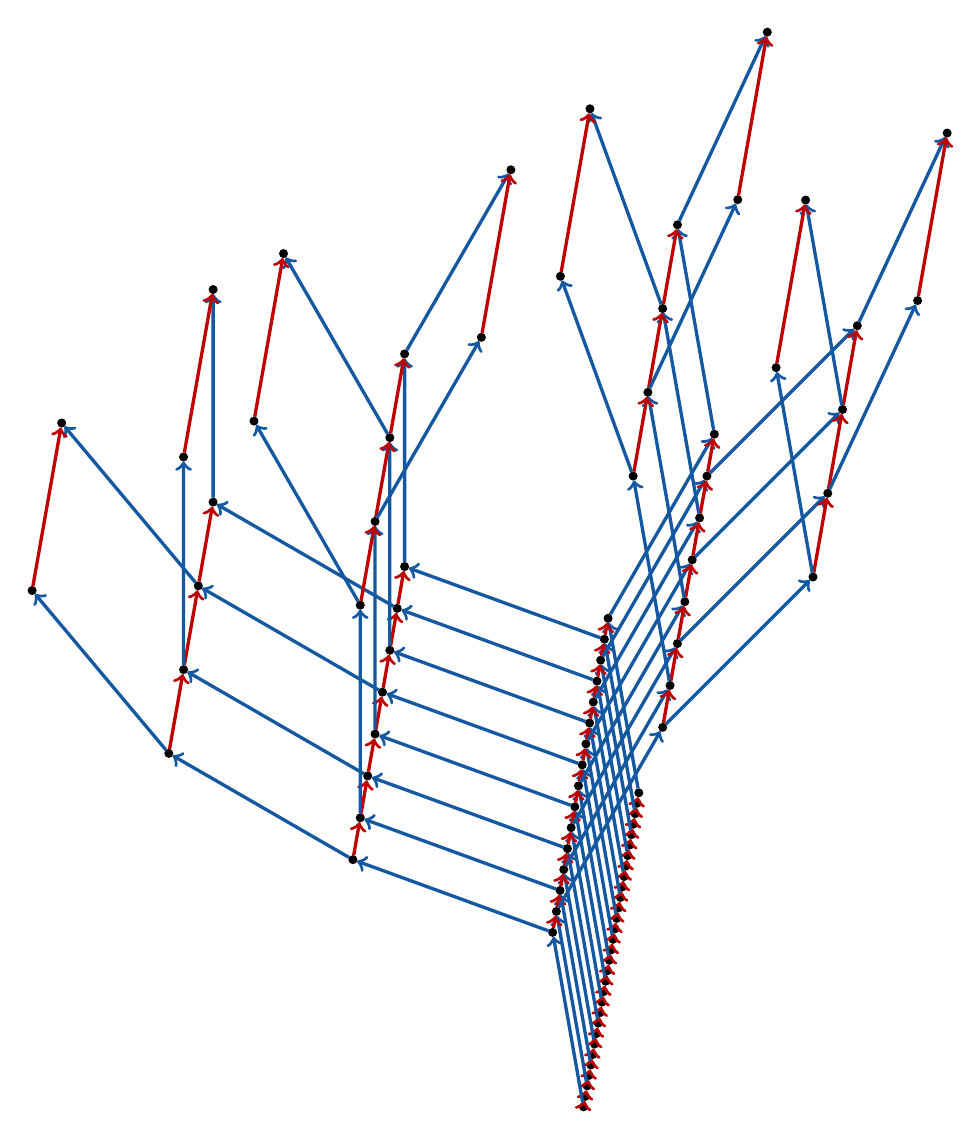
\begin{tikzpicture}
	[scale=0.45,node distance=0.5cm,
	nn/.style={circle,fill,draw=black,inner sep=1pt},font=\small]
	%%%%% LEVEL -1
	\node[nn] (nivelm10) at (0,0) {};
	\foreach \i[remember=\i as \lasti (initially 0)] in {1,...,30}
	{
	\node[nn] (nivelm1\i) at ([shift=({80:0.3 cm})]nivelm1\lasti) {};
	\path[->, very thick,draw={rgb, 255:red, 191; green, 0; blue, 0 }] (nivelm1\lasti) edge (nivelm1\i);
	};
	%%%%% LEVEL 0
	\foreach \i[remember=\i as \lasti (initially 0)] in {0,2,...,30}
	{
	\node[nn] (nivel0\i) at ([shift=({100:5 cm})]nivelm1\i) {};
	\path[->, very thick,draw={rgb, 255:red, 19; green, 88; blue, 160 }] (nivelm1\i) edge (nivel0\i);
	\ifnum \i>0
	\path[->, very thick,draw={rgb, 255:red, 191; green, 0; blue, 0 }] (nivel0\lasti) edge (nivel0\i);
	\fi 
	};
	%%%%% LEVEL 1
	\foreach \i[remember=\i as \lasti (initially 0)] in {0,4,...,30}
	{
	\node[nn] (nivel1\i) at ([shift=({160:6 cm})]nivel0\i) {};
	\path[->, very thick,draw={rgb, 255:red, 19; green, 88; blue, 160 }] (nivel0\i) edge (nivel1\i);
	\ifnum \i>0
	\path[->, very thick,draw={rgb, 255:red, 191; green, 0; blue, 0 }] (nivel1\lasti) edge (nivel1\i);
	\fi 
	};
	\foreach \i[remember=\i as \lasti (initially 2)] in {2,6,...,30}
{
	\node[nn] (nivel1\i) at ([shift=({60:6 cm})]nivel0\i) {};
	\path[->, very thick,draw={rgb, 255:red, 19; green, 88; blue, 160 }] (nivel0\i) edge (nivel1\i);
	\ifnum \i>2
	\path[->, very thick,draw={rgb, 255:red, 191; green, 0; blue, 0 }] (nivel1\lasti) edge (nivel1\i);
	\fi 
};
    %%%%% LEVEL 2
    \foreach \i[remember=\i as \lasti (initially 0)] in {0,8,...,30}
    {
    	\node[nn] (nivel2\i) at ([shift=({150:6 cm})]nivel1\i) {};
    	\path[->, very thick,draw={rgb, 255:red, 19; green, 88; blue, 160 }] (nivel1\i) edge (nivel2\i);
    	\ifnum \i>0
    	\path[->, very thick,draw={rgb, 255:red, 191; green, 0; blue, 0 }] (nivel2\lasti) edge (nivel2\i);
    	\fi 
    };
    \foreach \i[remember=\i as \lasti (initially 4)] in {4,12,...,30}
{
	\node[nn] (nivel2\i) at ([shift=({90:6 cm})]nivel1\i) {};
	\path[->, very thick,draw={rgb, 255:red, 19; green, 88; blue, 160 }] (nivel1\i) edge (nivel2\i);
	\ifnum \i>4
	\path[->, very thick,draw={rgb, 255:red, 191; green, 0; blue, 0 }] (nivel2\lasti) edge (nivel2\i);
	\fi 
};
    \foreach \i[remember=\i as \lasti (initially 2)] in {2,10,...,30}
{
	\node[nn] (nivel2\i) at ([shift=({45:6 cm})]nivel1\i) {};
	\path[->, very thick,draw={rgb, 255:red, 19; green, 88; blue, 160 }] (nivel1\i) edge (nivel2\i);
	\ifnum \i>2
	\path[->, very thick,draw={rgb, 255:red, 191; green, 0; blue, 0 }] (nivel2\lasti) edge (nivel2\i);
	\fi 
};
    \foreach \i[remember=\i as \lasti (initially 6)] in {6,14,...,30}
{
	\node[nn] (nivel2\i) at ([shift=({100:6 cm})]nivel1\i) {};
	\path[->, very thick,draw={rgb, 255:red, 19; green, 88; blue, 160 }] (nivel1\i) edge (nivel2\i);
	\ifnum \i>6
	\path[->, very thick,draw={rgb, 255:red, 191; green, 0; blue, 0 }] (nivel2\lasti) edge (nivel2\i);
	\fi 
};
	%%%% LEVEL 3
 \foreach \i[remember=\i as \lasti (initially 0)] in {0,16,...,30}
{
	\node[nn] (nivel3\i) at ([shift=({130:6 cm})]nivel2\i) {};
	\path[->, very thick,draw={rgb, 255:red, 19; green, 88; blue, 160 }] (nivel2\i) edge (nivel3\i);
	\ifnum \i>0
	\path[->, very thick,draw={rgb, 255:red, 191; green, 0; blue, 0 }] (nivel3\lasti) edge (nivel3\i);
	\fi 
};
 \foreach \i[remember=\i as \lasti (initially 2)] in {2,18,...,30}
{
	\node[nn] (nivel3\i) at ([shift=({100:6 cm})]nivel2\i) {};
	\path[->, very thick,draw={rgb, 255:red, 19; green, 88; blue, 160 }] (nivel2\i) edge (nivel3\i);
	\ifnum \i>2
	\path[->, very thick,draw={rgb, 255:red, 191; green, 0; blue, 0 }] (nivel3\lasti) edge (nivel3\i);
	\fi 
};
 \foreach \i[remember=\i as \lasti (initially 4)] in {4,20,...,30}
{
	\node[nn] (nivel3\i) at ([shift=({120:6 cm})]nivel2\i) {};
	\path[->, very thick,draw={rgb, 255:red, 19; green, 88; blue, 160 }] (nivel2\i) edge (nivel3\i);
	\ifnum \i>4
	\path[->, very thick,draw={rgb, 255:red, 191; green, 0; blue, 0 }] (nivel3\lasti) edge (nivel3\i);
	\fi 
};
 \foreach \i[remember=\i as \lasti (initially 6)] in {6,22,...,30}
{
	\node[nn] (nivel3\i) at ([shift=({110:6 cm})]nivel2\i) {};
	\path[->, very thick,draw={rgb, 255:red, 19; green, 88; blue, 160 }] (nivel2\i) edge (nivel3\i);
	\ifnum \i>6
	\path[->, very thick,draw={rgb, 255:red, 191; green, 0; blue, 0 }] (nivel3\lasti) edge (nivel3\i);
	\fi 
};
 \foreach \i[remember=\i as \lasti (initially 8)] in {8,24,...,30}
{
	\node[nn] (nivel3\i) at ([shift=({90:6 cm})]nivel2\i) {};
	\path[->, very thick,draw={rgb, 255:red, 19; green, 88; blue, 160 }] (nivel2\i) edge (nivel3\i);
	\ifnum \i>8
	\path[->, very thick,draw={rgb, 255:red, 191; green, 0; blue, 0 }] (nivel3\lasti) edge (nivel3\i);
	\fi 
};
 \foreach \i[remember=\i as \lasti (initially 10)] in {10,26,...,30}
{
	\node[nn] (nivel3\i) at ([shift=({65:6 cm})]nivel2\i) {};
	\path[->, very thick,draw={rgb, 255:red, 19; green, 88; blue, 160 }] (nivel2\i) edge (nivel3\i);
	\ifnum \i>10
	\path[->, very thick,draw={rgb, 255:red, 191; green, 0; blue, 0 }] (nivel3\lasti) edge (nivel3\i);
	\fi 
};
 \foreach \i[remember=\i as \lasti (initially 12)] in {12,28,...,30}
{
	\node[nn] (nivel3\i) at ([shift=({60:6 cm})]nivel2\i) {};
	\path[->, very thick,draw={rgb, 255:red, 19; green, 88; blue, 160 }] (nivel2\i) edge (nivel3\i);
	\ifnum \i>12
	\path[->, very thick,draw={rgb, 255:red, 191; green, 0; blue, 0 }] (nivel3\lasti) edge (nivel3\i);
	\fi 
};
 \foreach \i[remember=\i as \lasti (initially 14)] in {14,30}
{
	\node[nn] (nivel3\i) at ([shift=({65:6 cm})]nivel2\i) {};
	\path[->, very thick,draw={rgb, 255:red, 19; green, 88; blue, 160 }] (nivel2\i) edge (nivel3\i);
	\ifnum \i>14
	\path[->, very thick,draw={rgb, 255:red, 191; green, 0; blue, 0 }] (nivel3\lasti) edge (nivel3\i);
	\fi 
};
	\end{tikzpicture}
	\caption{A section of the Cayley graph of $BS(1,2)$.  Red edges are those labeled with ``$a$'', while blue edges are those labeled with ``$b$''.}
	\label{fig:cayley_bs}
\end{figure}

\begin{figure}
	\centering
	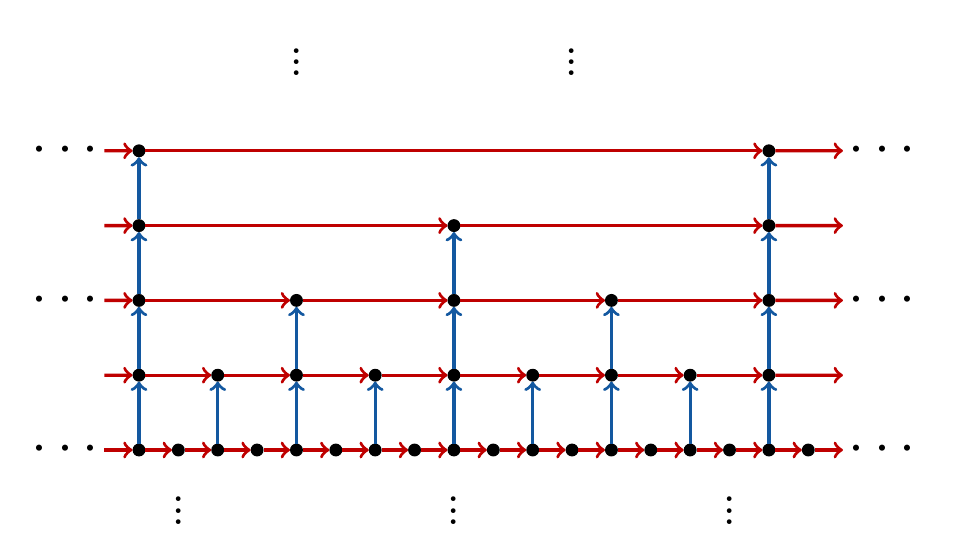
\begin{tikzpicture}
	[yscale=0.95,xscale=0.25,
	nn/.style={circle,fill,draw=black,inner sep=1.8pt},font=\small]
	\begin{scope}[auto, every node/.style={inner sep=1.5pt}]
	%LEVEL 0
	\node[font=\fontsize{20}{20}\selectfont] (leftdots) at (8,5.3) {$\vdots$};
	\node[font=\fontsize{20}{20}\selectfont] (leftdots) at (22,5.3) {$\vdots$};
	\node[font=\fontsize{20}{20}\selectfont] (leftdots) at (-3.5,0) {$\cdots$};
	\node[font=\fontsize{20}{20}\selectfont] (leftdots2) at (-3.5,4) {$\cdots$};
	\node[font=\fontsize{20}{20}\selectfont] (leftdots2) at (-3.5,2) {$\cdots$};
	\node[font=\fontsize{20}{20}\selectfont] (rightdots) at (38,0) {$\cdots$};	
	\node[font=\fontsize{20}{20}\selectfont] (rightdots) at (38,2) {$\cdots$};	
	\node[font=\fontsize{20}{20}\selectfont] (rightdots2) at (38,4) {$\cdots$};		
	\node[font=\fontsize{20}{20}\selectfont] (rightdots2) at (2,-0.7) {$\vdots$};	
	\node[font=\fontsize{20}{20}\selectfont] (rightdots2) at (16,-0.7) {$\vdots$};				
	\node[font=\fontsize{20}{20}\selectfont] (rightdots2) at (30,-0.7) {$\vdots$};							
	\foreach \x in {0,...,3}
	\node[shape=circle,draw=black,fill] (a\x) at (2*\x,0) {};
	\foreach \x in {4,...,7}
	\node[shape=circle,draw=black,fill] (a\x) at (2*\x,0) {};	
	\foreach \x in {8,...,11}
	\node[shape=circle,draw=black,fill] (a\x) at (2*\x,0) {};
	\foreach \x in {12,...,15}
	\node[shape=circle,draw=black,fill] (a\x) at (2*\x,0) {};			
	\foreach \x in {16,...,17}
	\node[shape=circle,draw=black,fill] (a\x) at (2*\x,0) {};
	\foreach \x in {0,...,16}
	\pgfmathtruncatemacro{\j}{\x+1}
	\path[->, very thick,draw={rgb, 255:red, 191; green, 0; blue, 0 }](a\x) edge node[below] {} (a\j);
	%LEVEL 1
	\foreach \x in {0,2,8,10,16}
	{
		\node[shape=circle,draw=black,fill] (a\x b) at (2*\x,1) {};
		\path[->,very thick,draw={rgb, 255:red, 19; green, 88; blue, 160 }](a\x) edge node[left] {} (a\x b);
	};
	\foreach \x in {4,6,12,14}
	{
		\node[shape=circle,draw=black,fill] (a\x b) at (2*\x,1) {};
		\path[->, very thick, draw={rgb, 255:red, 19; green, 88; blue, 160 }](a\x) edge node[left] {} (a\x b);
	};
	\foreach \x in {0,2,4,6,8,10,12,14}
	{
		\pgfmathtruncatemacro{\j}{\x+2}
		\path[->, very thick, draw = {rgb, 255:red, 191; green, 0; blue, 0 }](a\x b) edge node[below] {} (a\j b);
	};
	%LEVEL 2
	\foreach \x in {0,4,8,12,16}
	{
		\node[shape=circle,draw=black,fill] (a\x b2) at (2*\x,2) {};
		\path[->, very thick, draw={rgb, 255:red, 19; green, 88; blue, 160 }](a\x b) edge node[left] {} (a\x b2);
	};
	\foreach \x in {0,4,8,12}
	{
		\pgfmathtruncatemacro{\j}{\x+4}
		\path[->, very thick, draw={rgb, 255:red, 191; green, 0; blue, 0 }](a\x b2) edge node[below] {} (a\j b2);
	};
	%LEVEL 3
	\foreach \x in {0,8,16}
	{
		\node[shape=circle,draw=black,fill] (a\x b3) at (2*\x,3) {};
		\path[->, very thick, draw={rgb, 255:red, 19; green, 88; blue, 160 }](a\x b2) edge node[left] {} (a\x b3);
	};
	\foreach \x in {0,8}
	{
		\pgfmathtruncatemacro{\j}{\x+8}
		\path[->,very thick, draw={rgb, 255:red, 191; green, 0; blue, 0 }](a\x b3) edge node[below] {} (a\j b3);
	};
	%LEVEL 4
	\foreach \x in {0,16}
	{
		\node[shape=circle,draw=black,fill] (a\x b4) at (2*\x,4) {};
		\path[->, very thick, draw={rgb, 255:red, 19; green, 88; blue, 160 }](a\x b3) edge node[left] {} (a\x b4);
	};
	\path[->, very thick, draw={rgb, 255:red, 191; green, 0; blue, 0 }](a0b4) edge node[below] {} (a16b4);
	\node[] (f0) at (36,0) {};
	\path[->,very thick, draw={rgb, 255:red, 191; green, 0; blue, 0 }](a17) edge node[below] {} (f0);
	\node[] (f1) at (36,1) {};
	\path[->,very thick, draw={rgb, 255:red, 191; green, 0; blue, 0 }](a16b) edge node[below] {} (f1);
	\node[] (f2) at (36,2) {};
	\path[->,very thick, draw={rgb, 255:red, 191; green, 0; blue, 0 }](a16b2) edge node[left] {} (f2);
	\node[] (f3) at (36,3) {};
	\path[->,very thick, draw={rgb, 255:red, 191; green, 0; blue, 0 }](a16b3) edge node[below] {} (f3);
	\node[] (f4) at (36,4) {};
	\path[->,very thick, draw={rgb, 255:red, 191; green, 0; blue, 0 }](a16b4) edge node[below] {} (f4);
	
	\node[] (i0) at (-2,0) {};
	\path[<-,very thick, draw={rgb, 255:red, 191; green, 0; blue, 0 }](a0) edge node[left] {} (i0);
	\node[] (i1) at (-2,1) {};
	\path[<-,very thick, draw={rgb, 255:red, 191; green, 0; blue, 0 }](a0b) edge node[left] {} (i1);
	\node[] (i2) at (-2,2) {};
	\path[<-,very thick, draw={rgb, 255:red, 191; green, 0; blue, 0 }](a0b2) edge node[left] {} (i2);
	\node[] (i3) at (-2,3) {};
	\path[<-,very thick, draw={rgb, 255:red, 191; green, 0; blue, 0 }](a0b3) edge node[left] {} (i3);
	\node[] (i4) at (-2,4) {};
	\path[<-,very thick, draw={rgb, 255:red, 191; green, 0; blue, 0 }](a0b4) edge node[left] {} (i4);
	\end{scope}	
	\end{tikzpicture}
	\caption{A section of a sheet of the Cayley graph of $BS(1,2)$.  Red edges are those labeled with ``$a$'', while blue edges are those labeled with ``$b$''.}
	\label{fig:bssheet}
\end{figure}

The next lemma summarizes some of the consequences induced by the defining relation used in the standard presentation of $\BS$. Its elementary proof is by induction and is omitted. These additional relations will prove useful in establishing a normal form for $\BS$ below.

\begin{lemma}\label{bs.further_identifications} The unique relation $bab^{-1}=a^N$ used to define $\BS$ forces further identifications: for every $j\ge 0$ and $k\in \mathbb{Z}$ we have $b^{j}a^k=a^{kN^j}b^j$.
\end{lemma}
	 \subsection{Symbolic Dynamics on finitely generated groups}
Talk about symbolic dynamics on finitely generated groups. Topological entropy.
	%%%%%%%%%%%%%%%%%%%%%%%
	
	\section{Weak periodicity}\label{section.weak_periodicity}
	asdasd

	
	\subsection{A normal form for ascending HNN-extensions}\label{subsection.HNN_extensions_normal_form}
   An HNN-extension where $K=G$ and $H\le G$ is a subgroup (isomorphic to $G$) is commonly called an \emph{ascending HNN-extension}. For this kind of groups we can give a more detailed version of the normal form given in \ref{prop.hnn_general_normal_form} .

	
	\begin{proposition}[Normal form]\label{prop.normalform_hnn_particular}
		Let $G$ be a group isomorphic to one of its subgroups $H$, through and isomorphism $\psi:G\to H$. Then the ascending HNN-extension $G*_{\psi}$ has a normal form given by words of the form $$t^{-j}gt^{i}, \text{ for }i,j\ge 0, \ g\in G,$$
		and such that $g\in H$ is only possible if $i=0$ or $j=0$.
	\end{proposition}
\begin{proof}
	Using the normal form for HNN-extensions described in Proposition \ref{prop.hnn_general_normal_form} with sets of representatives $T_G=\{e_G\}$ and $T_H$ containing $e_G$, we distinguish two types of words.
	
	\begin{enumerate}[1.]
		\item The first type are words of the form $g_0t^i$, for $g_0\in G$, $i\ge 0$. This word is already in the form described in the proposition so in this case we are finished.
		\item The second type are words of the form $g_0t^{-1}g_1\cdots t^{-1}g_n$, for $g_0\in G$, $g_1,\ldots,g_n\in T_H$. We will prove we can arrive at the normal form described in the proposition by induction. Moreover we will prove that there exists $\tilde{g}\in G$ such that $g_0t^{-1}g_1\cdots t^{-1}g_n=t^{-n}\psi(\tilde{g})g_n$. If $n=1$, then we can use the relation from the HNN-extension to obtain
		$$
		g_0t^{-1}g_1=t^{-1}\psi^(g_0)g_1.
		$$
		In the general case for $n\ge 2$, by the induction hypothesis we know that for some $\tilde{g}\in G$ we have $$g_0t^{-1}g_1\cdots t^{-1}g_{n-1}=t^{-(n-1)}\psi(\tilde{g})g_{n-1}.$$
		
		Then
		\begin{align*}
		g_0t^{-1}g_1\cdots t^{-1}g_n&=t^{-(n-1)}\psi(\tilde{g})g_{n-1}t^{-1}g_n\\
		&=t^{-n}\psi(\tilde{g}g_{n-1})g_n,
		\end{align*}
		finishing the induction.
		\item Finally, the third type are words of the form $g_0t^{-1}g_1\cdots t^{-1}g_nt^{j}$, for $g_0\in G$, $g_1,\ldots,g_n\in T_H$ and $j\ge 1$. Proceeding as in the previous case, we show that there must exist $\tilde{g}\in G$ such that.
		$$
		g_0t^{-1}g_1\cdots t^{-1}g_nt^{j}=t^{-n}\psi(\tilde{g})g_{n}t^{j}
		$$
		
		Note that as $j\ge 1$, the conditions from Proposition \ref{prop.hnn_general_normal_form} ensures that $g_n\in T_H\backslash\{e_G \}$ (since otherwise the considered word would contain a subword of the form $t^{-1}e_Gt$, which is forbidden), and hence $\psi(\tilde{g})g_{n}\notin H$.
	\end{enumerate}
\end{proof}
Describe Cayley graph and interpret normal form through it. 


Considering ------- we deduce a normal form for amenable non-abelian Baumslag-Solitar groups.

\begin{corollary}\label{prop.normalform_bsgroups}
	The amenable non-abelian Baumslag-Solitar groups $\BS$, $N\ge 2$, have a normal form given by words $b^{-j}a^kb^{i}$ where $i,j\ge 0$ and $k\in \mathbb{Z}$, and $k$ may be divisible by $N$ only if $i=0$ or $j=0$.
\end{corollary}

	\subsection{Weak $H$-periodicity}\label{subsection.weak_H_periodicity}
	
	

	\subsection{The case of amenable non-abelian Baumslag-Solitar groups}\label{subsection.BS_periodicity}
	This chapter is focused on studying how periodic configurations on $\mathcal{A}^{\BS}$ exhibit a sort of rigidity when their stabilizer and the structure of the Cayley graph of the group synchronize in some sense. In particular, we will study weak periodicity in the $a$-direction and obtain results regarding the structure of $a$-rows of configurations with this periodicity.
	
	
	We start by giving the following definition fo the $a$-rows of $\BS$, which are the subsets that look like a copy of $\mathbb{Z}$ in the direction of the generator $a$ of the Cayley graph.
	\begin{definition}For $g\in \BS$ we define the \textbf{$a$-row containing $g$} as 
		$$
		\Gamma_g\coloneqq\{ ga^m\mid m\in \mathbb{Z}\}.
		$$
		Using the normal form to write $g=b^{-j}a^kb^i$, for $i,j\ge 0$ and $k\in \mathbb{Z}$ such that $k\in N\mathbb{Z}$ is only possible if $ij=0$, we say that $\Gamma_g$ is an \textbf{$a$-row at level } $i-j$. Note that since the normal form of an element is unique, the level of the corresponding $a$-row $\Gamma_g$ is well defined.
	\end{definition}
	\begin{remark*} Given an element $g=b^{-j}a^kb^i\in \BS$ written in its normal form, we have that for any $m\in \mathbb{Z}$:
		\begin{equation*}
		ga^m=b^{-j}a^kb^ia^m=b^{-j}a^{k+mN^i}b^i.
		\end{equation*}
		Then the $a$-row $\Gamma_g$ has an alternative description given by
		$$
		\Gamma_g=\left\{b^{-j}a^{k+mN^i}b^i\mid  m\in \mathbb{Z}  \right\},
		$$
		which has the advantage of showing in a clearer way which elements (written in their normal form) are adjacent to each other in the Cayley graph through an edge labeled by the $a$-generator.
	\end{remark*}
	
%	Suppose we have a configuration $x\in \mathcal{A}^{\BS}$ such that $a^N\in \mathrm{Stab}(x)$. This periodicity translates to the fact that the configuration stays the same by translating the Cayley graph of $\BS$ $N$ steps in the $a$-direction. Interpreting $x|_{\Gamma_{e_{\BS}}}$ as a biinfinite sequence in $\mathcal{A}^\mathbb{Z}$ we have that $N\in \mathrm{Stab}(x|_{\Gamma_{e_{\BS}}})$, and moreover we must have that $e_{\BS}\in\mathrm{Stab}(x|_{\Gamma_{b}})$ and $e_{\BS}\in \mathrm{Stab}(x|_{\Gamma_{ab}})$, from which we see that $x$ can only have one symbol of the alphabet on each of the $a$-rows $\Gamma_{b}$ and $\Gamma_{ab}$. Figure \ref{fig:aNinStabx} illustrates this with $N=2$, where we see that the first $a$-row exhibits period $2$ on its symbols, and with it the next $a$-rows in the sheets originating from this base are forced to have period $1$.
%	\begin{figure}[H]
%		\centering
%		\begin{tikzpicture}[xscale=0.5,yscale=1.1]
%		\begin{scope}[auto, every node/.style={inner sep=2}]
%		%LEVEL 0
%		\foreach \x in {0,2,4,6,8}
%		\node[shape=circle,draw=black,fill=red!50] (a\x) at (2*\x,0) {$\alpha_1$};
%		\foreach \x in {1,3,5,7,9}
%		\node[shape=circle,draw=black,fill=cyan!50] (a\x) at (2*\x,0) {$\alpha_2$};
%		\foreach \x in {0,...,8}
%		\pgfmathtruncatemacro{\j}{\x+1}
%		\path[-, thick](a\x) edge node[left] {} (a\j);
%		%LEVEL 1
%		\foreach \x in {0,2,4,6,8}
%		{
%			\node[shape=circle,draw=black,fill=black!10!green!60] (a\x b) at (2*\x,1) {$\alpha_3$};
%			\path[-, thick](a\x b) edge node[left] {} (a\x);
%		};
%		\foreach \x in {0,2,4,6}
%		{
%			\pgfmathtruncatemacro{\j}{\x+2}
%			\path[-, thick](a\x b) edge node[left] {} (a\j b);
%		};
%		\foreach \x in {1,3,5,7,9}
%		{
%			\node[shape=circle,draw=black,fill=magenta!50] (a\x b) at (2*\x,2) {$\alpha_4$};
%			\path[-, thick](a\x b) edge node[left] {} (a\x);
%		};
%		\foreach \x in {1,3,5,7}
%		{
%			\pgfmathtruncatemacro{\j}{\x+2}
%			\path[-, thick](a\x b) edge node[left] {} (a\j b);
%		};
%		\end{scope}	
%		\end{tikzpicture}
%		\caption{Example of a configuration $x$ with $a^N\in \mathrm{Stab}(x)$.}
%		\label{fig:aNinStabx}
%	\end{figure}	
%	Now suppose instead we have a point $x\in \mathcal{A}^{\BS}$ such that $a^{N^2}\in \mathrm{Stab}(x)$. Similarly to the above case, using the relation of the group $\BS$ we see that the sequences $x|_{\Gamma_{e_{\BS}}}, x|_{\Gamma_{b}}$ and $x|_{\Gamma_{b^2}}$ must have periods $N^2,N$ and $1$, respectively. This is illustrated in Figure \ref{fig:aN2inStabx} showing part of a sheet of the Cayley graph of $\BS[2]$, where the base $a$-row has period $4=2^2$, the one above it has period $2=2^1$ and the next one period $1=2^0$.
%	\begin{figure}[H]
%		\centering
%		\begin{tikzpicture}[xscale=0.5,yscale=1]
%		\begin{scope}[auto, every node/.style={inner sep=2}]
%		%LEVEL 0
%		\foreach \x in {0,4,8,12}
%		\node[shape=circle,draw=black,fill=red!50] (a\x) at (2*\x,0) {$\alpha_1$};
%		\foreach \x in {1,5,9}
%		\node[shape=circle,draw=black,fill=orange!50] (a\x) at (2*\x,0) {$\alpha_2$};
%		\foreach \x in {2,6,10}
%		\node[shape=circle,draw=black,fill=yellow!50] (a\x) at (2*\x,0) {$\alpha_3$};
%		\foreach \x in {3,7,11}
%		\node[shape=circle,draw=black,fill=black!10!green!60] (a\x) at (2*\x,0) {$\alpha_4$};
%		\foreach \x in {0,...,11}
%		\pgfmathtruncatemacro{\j}{\x+1}
%		\path[-, thick](a\x) edge node[left] {} (a\j);
%		%LEVEL 1
%		\foreach \x in {0,4,8,12}
%		{
%			\node[shape=circle,draw=black,fill=cyan!50] (a\x b) at (2*\x,1.5) {$\alpha_5$};
%			\path[-, thick](a\x b) edge node[left] {} (a\x);
%		};
%		\foreach \x in {2,6,10}
%		{
%			\node[shape=circle,draw=black,fill=magenta!50] (a\x b) at (2*\x,1.5) {$\alpha_6$};
%			\path[-, thick](a\x b) edge node[left] {} (a\x);
%		};
%		\foreach \x in {0,2,4,6,8,10}
%		{
%			\pgfmathtruncatemacro{\j}{\x+2}
%			\path[-, thick](a\x b) edge node[left] {} (a\j b);
%		};
%		%LEVEL 2
%		\foreach \x in {0,4,8,12}
%		{
%			\node[shape=circle,draw=black,fill=black!10!green!60] (a\x b2) at (2*\x,3) {$\alpha_7$};
%			\path[-, thick](a\x b2) edge node[left] {} (a\x b);
%		};
%		\foreach \x in {0,4,8}
%		{
%			\pgfmathtruncatemacro{\j}{\x+4}
%			\path[-, thick](a\x b2) edge node[left] {} (a\j b2);
%		};
%		\end{scope}	
%		\end{tikzpicture}
%		\caption{Example of a configuration $x$ with $a^{N^2}\in \mathrm{Stab}(x)$.}
%		\label{fig:aN2inStabx}
%	\end{figure}
%	
%	The behaviour found in the previous examples may be stated as the fact that a configuration having an $N$-th power of $a$ in its stabilizer is forced to have $a$-rows sufficiently high in the $b$-direction which are all monochromatic, in the sense that they have the same symbol repeated over and over again.
%	\begin{proposition} \label{prop:monochrom_col_easycase}
%		Let $x\in \mathcal{A}^{\BS}$ and $\ell\ge 0$ be such that $\sigma_{a^{N^{\ell}}}(x)=x$. Then every $a$-row at a level greater or equal than $\ell$ in $x$ is monochromatically colored. That is, for every $i,j\ge 0$ and $m, k\in \mathbb{Z}$:
%		$$
%		x_{b^{-j}a^kb^{j+i+\ell}}=x_{b^{-j}a^kb^{j+i+\ell}a^m}.
%		$$
%		Moreover, for every $i\ge \ell$ and $h\ge 1$ all the $a$-rows at level $i+h$ sharing a common base of level $i$ in $x$ are equal. Formally this means that for every $j\ge 0$, $k\in \mathbb{Z}$ and $q\in \{0,\ldots,N^h-1\}$:
%		$$
%		x_{b^{-j}a^{k}b^{j+i+h}}=x_{b^{-j}a^{k}b^{j+i}a^{q}b^{h}}
%		$$
%	\end{proposition}
%	Under the further assumption that $x$ is a strongly periodic point we see that the behaviour seen in the previous proposition is extended to the entire group, allowing each $a$-row to only have one symbol on it.
%	\begin{corollary}\label{cor:monochromatic_rows_easy}Let $x\in \mathcal{A}^{\BS}$ be a strongly periodic configuration such that $\exists \ell\ge 0: \sigma_{a^{N^{\ell}}}(x)=x.$ Then for every $g\in \BS$ the $a$-row $\Gamma_g$ is monochromatically colored by $x$. That is, for every $m_1,m_2\in \mathbb{Z}$:
%		$$
%		x_{ga^{m_1}}=x_{ga^{m_2}}.
%		$$
%	\end{corollary}
%	\begin{corollary} Let $X\subseteq \mathcal{A}^{\BS}$ be a $\BS$-subshift and $x\in X$ such that there exists $\ell\ge 0$ such that $\sigma_{a^{N^\ell}}(x)=x$. Then there exists a configuration $y\in X$ such that each of its $a$-rows is monochromatic, and all $a$-rows of the same level in $y$ are equal. Moreover, if $X$ is an SFT then $y$ can be chosen to be strongly periodic.
%	\end{corollary}
%	\begin{remark*} Having all $a$-rows monochromatic is not a sufficient condition for a configuration $x\in \mathcal{A}^{\BS}$ to be strongly periodic. One can construct an example of such a configuration by considering a non-periodic sequence $z\in \mathcal{A}^\mathbb{Z}$ and define $x\in x\in \mathcal{A}^{\BS}$ to consist of monochromatic $a$-rows whose symbols are defined according to the sequence $z$. Figure \ref{fig:monochromatic_rows_tree_counterexample} shows a sideways view of the Cayley graph of $\BS$, where each symbol in this figure represents the symbol of the entire $a$-row at that level in $x$.
%		\begin{figure}[H]
%			\centering
%			\begin{tikzpicture}[grow'=up]
%			\begin{scope}
%			\clip (-5,0.3) rectangle (5,6);
%			\Tree [.$z_{-2}$ [.$z_{-1}$ [.$z_{0}$ [.$z_{1}$ [.$z_{2}$ $\vdots$ ] [.$z_{2}$ $\vdots$ ] ] [.$z_{1}$ [.$z_{2}$ $\vdots$ ] [.$z_{2}$ $\vdots$ ] ] ] [.$z_{0}$ [.$z_{1}$ [.$z_{2}$ $\vdots$ ] [.$z_{2}$ $\vdots$ ] ] [.$z_{1}$ [.$z_{2}$ $\vdots$ ] [.$z_{2}$ $\vdots$ ] ] ] ]];
%			\end{scope}
%			\node[very thick] at (0,0) {$\vdots$};
%			\end{tikzpicture}
%			\caption{Illustration of a configuration in a sideways view of the Cayley graph of $\BS$, having all $a$-rows monochromatic but not being strongly periodic.}
%			\label{fig:monochromatic_rows_tree_counterexample}
%		\end{figure}
%	\end{remark*}
%	
	Similar results to the ones proved above can be obtained if one considers the broader class of weakly periodic configurations $x\in \mathcal{A}^{\BS}$ such that $\sigma_{a^{pN^\ell}}(x)=x$, for $\ell\ge 0$ and $p\notin N\mathbb{Z}$. In the remainder of this section we make this generalization, using the same ideas found in the proofs above.
	
	\begin{proposition}\label{prop.bs_periodicity_p_generalcase}
		Let $x\in \mathcal{A}^{\BS}$, $\ell\ge 0$ and $p\notin N\mathbb{Z}$ be such that $\sigma_{a^{pN^\ell}}(x)=x$. Then every $a$-row of level greater or equal than $\ell$ is $p$-periodic, that is, for every $i,j\ge 0$, $k,m\in \mathbb{Z}$:
		$$
		x_{b^{-j}a^kb^{j+i+\ell}a^{m+p}}=x_{b^{-j}a^kb^{j+i+\ell}a^{m}}.
		$$
		Moreover, if we further assume that $\gcd(p,N)=1$, then for every $i\ge \ell$ and $h\ge 0$ all the $a$-rows of level $i+h$ sharing a common base $a$-row of level $i$ are equal, up to a translation. More precisely, for every $h\ge 0$ there exists $r\in \mathbb{Z}$ such that for every $j\ge 0$, $i\ge \ell$, $k,m\in \mathbb{Z}$ and $q\in \{0,\ldots,N^h-1\}$:
		$$
		x_{b^{-j}a^{k}b^{j+i+h}a^{m}}=x_{b^{-j}a^{k}b^{j+i}a^{q}b^{h}a^{m-qr}}.
		$$
		
	\end{proposition}
	\begin{proof}
		Note that for $i,j\ge 0$ and $k,m\in \mathbb{Z}$ we have that
		\begin{align*}
		b^{-j}a^kb^{j+i+\ell}a^{m+p}&=b^{-j}a^ka^{pN^{j+i+\ell}}b^{j+i+\ell}a^{m}\\
		&=b^{-j}a^{pN^{i+\ell}N^j}a^{k}b^{j+i+\ell}a^{m}\\
		&=a^{pN^{i+\ell}}b^{-j}a^{k}b^{j+i+\ell}a^{m}\\
		&=a^{N^{i}pN^{\ell}}b^{-j}a^{k}b^{j+i+\ell}a^{m}.
		\end{align*}
		As $\sigma_{a^{pN^{\ell}}}(x)=x$ we also have that $\sigma_{a^{N^{i}pN^{\ell}}}(x)=x$ and with it
		\begin{align*}
		x_{b^{-j}a^kb^{j+i+\ell}a^{m+p}}&=x_{a^{N^{i}pN^{\ell}}b^{-j}a^{k}b^{j+i+\ell}a^{m}}\\
		&=x_{b^{-j}a^{k}b^{j+i+\ell}a^{m}}.
		\end{align*}
		This proves that every $a$-row of level greater or equal than $\ell$ is $p$-periodic, seen as a bi-infinite sequence.
		
		For the second part of the proposition, note that as we assume that $\gcd(p,N)=1$ then for every $h\ge 1$ we have $\gcd(p,N^h)=1$ and hence by Bézout's identity there exist $r,s\in \mathbb{Z}$ such that $1=sp+rN^h$. With this we get that for $j\ge 0$, $i\ge \ell$, $k,m\in \mathbb{Z}$ and $q\in \{0,\ldots,N^h-1\}$:
		\begin{align*}
		b^{-j}a^{k}b^{j+i}a^{q}b^{h}a^{m-qr}&=b^{-j}a^{k}b^{j+i}a^{q}a^{-qrN^h}b^{h}a^{m}\\
		&=b^{-j}a^{k}b^{j+i}a^{q-qrN^h}b^{h}a^{m}\\
		&=b^{-j}a^{k}a^{q(1-rN^{h})N^{i+j}}b^{j+i}b^{h}a^{m}\\
		&=b^{-j}a^{q(1-rN^{h})N^{i}N^{j}}a^{k}b^{j+i}b^{h}a^{m}\\	
		&=a^{q(1-rN^{h})N^{i}}b^{-j}a^{k}b^{j+i}b^{h}a^{m}\\
		&=a^{qspN^{i-\ell}N^{\ell}}b^{-j}a^{k}b^{j+i}b^{h}a^{m}\\
		&=a^{qsN^{i-\ell}pN^{\ell}}b^{-j}a^{k}b^{j+i}b^{h}a^{m}.				
		\end{align*}
		Then as $\sigma_{a^{pN^\ell}}(x)=x$ we also have that $\sigma_{a^{qsN^{i-\ell}pN^{\ell}}}(x)=x$ and hence
		\begin{align*}
		x_{b^{-j}a^{k}b^{j+i}a^{q}b^{h}a^{m-qr}}&=x_{a^{qsN^{i-\ell}pN^{\ell}}b^{-j}a^{k}b^{j+i}b^{h}a^{m}}\\
		&=x_{b^{-j}a^{k}b^{j+i}b^{h}a^{m}}.
		\end{align*}
		The above proves that all $a$-rows $\Gamma_{b^{-j}a^kb^{j+i}a^qb^h}$ (for $q\in \{0,\ldots,N^h-1\}$) at level $i+h$, originating from the $a$-row $\Gamma_{b^{-j}a^kb^{j+i}}$ have the same sequence in $x$, namely $\{x_{b^{-j}a^{k}b^{j+i}b^{h}a^{m}}\}_{m\in \mathbb{Z}}$, up to a translation of $qr$.
	\end{proof}
	
	\begin{remark*} The second part of the previous propositon still holds if one does not assume that $\gcd(p,N)=1$, with the slight alteration of requiring $i\ge \ell+1$ instead of $i\ge \ell$. To prove this it is sufficient to note that $\sigma_{a^{pN^\ell}}(x)=x$ and $d\coloneqq \gcd(p,N)$, then we also have $\sigma_{a^{\frac{N}{d}pN^\ell}}(x)=x$ and hence 
		$$
		\sigma_{a^{\frac{p}{d}N^{\ell+1}}}(x)=x,
		$$
		from which we can apply Proposition \ref{prop.bs_periodicity_p_generalcase}.
	\end{remark*}
	
	\begin{corollary} Let $x\in \mathcal{A}^{\BS}$ be a strongly periodic configuration such that there exists $\ell\ge 0$ such that $\sigma_{a^{N^{\ell}}}(x)=x.$ Then for every $g\in \BS$ the $a$-row $\Gamma_g$ in $x$ has period $p$. That is, for every $m\in \mathbb{Z}$:
		$$
		x_{ga^{m}}=x_{ga^{m+p}}.
		$$
	\end{corollary}
	\begin{proof}
		Since $x$ is strongly periodic, it has a finite orbit under the action of $\BS$, so in particular the set $\{ \sigma_{b^{-q}}(x): q\ge 1 \}$ is finite. Hence there exists a sequence of increasing positive integers $\{q_n\}_{n\ge 1}$ such that for every $n\ge1$
		$$
		\sigma_{b^{-q_1}}(x)=\sigma_{b^{-q_n}}(x),
		$$
		or equivalently
		$$
		\sigma_{b^{q_1-q_n}}(x)=x.
		$$
		By taking $n$ sufficiently large, one can find $k\ge \ell $ and $j\in\left\{0,\ldots,N-1\right\}^k$ such that $b^{q_n-q_1}g\in \Gamma_{k}^{(j)}$ and using Proposition \ref{prop.bs_periodicity_p_generalcase} we see that for $m\ge 1:$
		\begin{equation*}
		\begin{aligned}
		x_{ga^{m}}&=(\sigma_{b^{q_1-q_n}}(x))_{ga^{m}} \\
		&=x_{b^{q_n-q_1}ga^{m}}\\
		&=x_{b^{q_n-q_1}ga^{m+p}} \\
		&=(\sigma_{b^{q_1-q_n}}(x))_{ga^{m+p}}\\
		&=x_{ga^{m+p}}.
		\end{aligned}
		\end{equation*}
		Hence every $a$-row $\Gamma_g$ in $x$ is a sequence of period $p$.
	\end{proof}
	\begin{corollary}
		Let $X\subseteq \mathcal{A}^{\BS}$ be a $\BS$-subshift and $x\in X$ such that there exist $\ell\ge 0$ and $p\notin N\mathbb{Z}$ such that $\sigma_{a^{pN^\ell}}(x)=x$. Then there exists a configuration $y\in X$ such that each of its $a$-rows is $p$-periodic, and all $a$-rows of the same level in $y$ are equal (up to translation). 
	\end{corollary}
	\begin{proof}
		Thanks to Proposition \ref{prop.bs_periodicity_p_generalcase} we have that all $a$-rows at a level greater or equal than $\ell$ in $x$ are $p$-periodic. We define for each $n\ge 1$ the configuration $x^n\coloneqq\sigma_{b^{-n}}(x)\in X$ and define $y\in X$ to be a limit point of the sequence $\{x^n\}_{n\in \mathbb{N}}$, which exists by compactness of $X$. 
		
		
		As each $a$-row at a sufficiently high level of $x$ is $p$-periodic and $a$-rows of the same level sharing a common base of a sufficiently high level in $x$ are equal, the construction of the sequence $\{x^n\}_{n\in \mathbb{N}}$ immediately shows that $y$ satisfies the required properties.
		\iffalse
		Now suppose that $X$ is an SFT. As periodicity is preserved through a conjugacy map, we may suppose without loss of generality that $X$ is a NNSFT. The pigeonhole principle guarantees that for the configuration $y$ from above, there are two levels which have the same $p$-periodic sequence in its rows. That is, there exists $h\ge 1$ (and with it $r\in \mathbb{Z}$) such that
		$$
		y_{a^k}=y_{a^{q}b^{h}a^{k-qr}},\ \forall k\in \mathbb{Z}, \ q\in \{0,\ldots,N^h-1\}.
		$$
		
		Now let us define a new configuration $z\in \mathcal{A}^{\BS}$, which copies the pattern seen in $y|_{\{a^kb^j\mid k\in \mathbb{Z}, 0\le j<h \}}$ throughout the group. This is done by defining:
		\begin{itemize}
			\item For $k\in \mathbb{Z}$, $i\in \{0,\ldots,h-1\}$,
			$$
			z_{a^kb^i}=y_{a^kb^i}.
			$$
			\item For $k\in \mathbb{Z}$, $i\in \{0,\ldots,h-1\}$, $f\ge 1$ and $q_0,\ldots,q_{f-1}\in \{0,\ldots,N^h-1\}$,
			$$
			z_{a^{q_0+q_1N^h+\cdots+q_{f-1}N^{(f-1)h}}b^{fh}a^kb^i}=y_{a^{k+(q_0+q_1+\ldots+q_{f-1})r}b^i}.
			$$
			
			\item For $w\ge 1$, $k\in \mathbb{Z}$ and $i\ge 0$,
			$$
			z_{b^{-wh}a^kb^i}=z_{a^kb^i}.
			$$
		\end{itemize}
		This definition is consistent and, thanks to the choice of $h$ and $r$ and the fact that $X$ is a NNSFT, we conclude that $z\in X$. Then $z$ is strongly periodic and 
		$$
		\mathrm{Orb}(z)=\{\sigma_{a^ib^j}\mid 0\le i<pN^h, \ 0\le j<h \}.
		$$
		\fi 
	\end{proof}
	
	
	
	
	
	\section{Graph-coloring subshifts}\label{section.graph_coloring_subshifts}
Given a group $G$ generated by a finite subset $S\subseteq G$ it is interesting to study the properties of proper colorings (in the sense used commonly in graph theory) of its Cayley graph. In this spirit we define for $n\ge 2$ the \textbf{graph-coloring subshift} (GCS)
$$
\mathcal{C}_{n}\coloneqq\left\{x\in \{0,\ldots,n-1\}^G\mid (\forall g\in G)(\forall s\in S)\ x_{g}\neq x_{gs} \right\},
$$
that is, for each configuration $x\in \mathcal{C}_{n}$ we have that $x$ describes a proper coloring of the Cayley graph $\Gamma(G,S)$ of $G$ with respect to the generator $S$. 
The subshift $\mathcal{C}_{n}$ is always an SFT, since it can be described by the finite set of forbidden patterns 
$$
\mathcal{F}\coloneqq \left\{ \{x_{e_G}=i,x_{s}=i\}\mid i\in \{0,\ldots,n-1\}, s\in S \right\}.
$$
The easiest case to study is $G=\mathbb{Z}$: since the Cayley graph of $\mathbb{Z}$ with respect to the generator $S=\{1\}$ is bipartite (see Example \ref{example:Cayley_graphs}), then $\mathcal{C}_n\neq \emptyset$ for every $n\ge 2$ and the number of words of length $m$ of $\mathcal{C}_{n}$ is $|\mathcal{L}_m(\mathcal{C}_{n})|=n(n-1)^{m-1}$. From this last equality we see that the topological entropy of $\mathcal{C}_n$ is 
$$\htop(\mathcal{C}_n)=\lim_{m\to \infty}\frac{1}{m}\log(n(n-1)^{m-1})=\log(n-1).$$
Note that in the case $n=2$ the subshift $\mathcal{C}_2$ only has two configurations. Nonetheless, starting from 3 colors the dynamics of this subshift becomes more interesting: for $n\ge 3$ the subshift $\mathcal{C}_n$ is topologically mixing. In fact, we can prove that given any two words $w_1,w_2\in \mathcal{L}(\mathcal{C}_n)$ and $M\ge 1$, we can find a pattern $u\in \mathcal{L}(\mathcal{C}_n)$ with $|u|=M+|w_1|+|w_2|$, $u|_{[1,|w_1|]}=w_1$ and $u|_{[M+|w_1|+1,M+|w_1|+|w_2|]}=w_2$: let $i$ and $j$ be the last symbols appearing in $w_1$ and $w_2$, respectively. If $i=j$, choose $k,l\in \{0,\ldots,n-1\}\backslash\{i\}$, $k\neq l$, and define $u\coloneqq w_1(kl)^\frac{M}{2}w_2$ if $M$ is even, and $u\coloneqq w_1(kl)^{\left\lfloor\frac{M}{2}\right\rfloor}kw_2$ if $M$ is odd. In the other case, that is if $i\neq j$, choose $k\in \{,\ldots,n-1\}\backslash\{i,j\}$ and define $u\coloneqq w_1(ki)^{\frac{M}{2}}w_2$ if $M$ is even and $u\coloneqq w_1(ki)^{\left\lfloor \frac{M}{2}\right \rfloor}kw_2$ if $M$ is odd. It is straightforward to check that said $u$ satisfies the claimed property in each case.

Another case of interest is $G=\mathbb{Z}^2$, or more generally $G=\mathbb{Z}^d$ for $d\ge 2$. Proper colorings of these groups have been studied recently, for example in \cite{alon2019mixing} and \cite{peled2018rigidity}. The latter of these two papers concerns mixing properties for colorings of $\mathbb{Z}^d$, where the authors define the notion of a frozen $q$-coloring of $\mathbb{Z}^d$ as a coloring with $q$ colors such that it cannot be modified on any finite subset to create a different coloring, and prove that $\mathbb{Z}^d$ admits frozen $q$-colorings if and only if $2\le q\le d+1$. They also prove that for $q\ge d+2$ any $q$-coloring of the boundary of the rectangle $\{1,\ldots,n\}^d$ for $n\ge d+2$ can be extended to a $q$-coloring of the entire box, and that if $q\ge 2d+1$ this can be done for every $n\ge 1$, therefore classifying all $q$-colorings of $\mathbb{Z}^d$ in terms of the properties with respect to the extensibility of patterns they exhibit.


The purpose of this section is to study the case $G=\BS$. We start by addressing the (non-)emptiness of the GCS $\mathcal{C}_n$ depending on the values of $N$ and $n$. Then we study the extensibility of locally admissible patterns, and later use it to give bounds for the topological entropy of $\mathcal{C}_n$. Finally we ask and answer partially the question of which mixing properties these $\BS$-subshifts possess.
The first question one should ask after making the definition of a GCS is whether this subshift is empty or not, that is, for which $n\ge 2$ the Cayley graph of $\BS$ admits a proper $n$-coloring. As we see in the next proposition, the answer to this question in the case of two colors depends on the parity of $N$, meanwhile for a number of colors $n\ge 3$ we have non-emptiness for every $N\ge 2$.

In what follows we consider the GCS in $n\ge 2$ colors for $\BS$ with respect to the generator $S=\{a,b\}$.

\begin{proposition}\label{prop.GCS_nonemptiness} If $N$ is odd $\mathcal{C}_2\neq \emptyset$, and if $N$ is even then $\mathcal{C}_2=\emptyset$ meanwhile $\mathcal{C}_3\neq \emptyset$. With this for every $N\ge 2$ and $n\ge 3$ we have $\mathcal{C}_n\neq \emptyset$.
\end{proposition}
\begin{proof}
	Let us see first that if $N$ is even then $\mathcal{C}_2=\emptyset$. To see this suppose we have $x\in \mathcal{C}_2$ and without loss of generality let us suppose that $x_{e_G}=0$. Then by the coloring rules we must have $x_{a^{N}}=0$, and $x_{b}=x_{a^Nb}=1$, but this cannot be since $x_{a^Nb}=x_{ba}$, so the neighboring vertices $b$ and $ba$ have the same color and this contradicts the GCS's definition.
	
	
	Now let us show that if $N$ is odd then $\mathcal{C}_2\neq \emptyset$. Moreover, we will show that in fact $|\mathcal{C}_2|=2$. To create a point $x\in \mathcal{C}_2$ let us impose that $x_{e_{\BS}}=0$, and define for every $g\in \BS$ expressed in its normal form $g=b^{-j}a^kb^i$ with $i,j\ge 0$ and $k\in \mathbb{Z}$: $x_g=i+j+k \mod 2$. We check that this provides a consistent coloring of the Cayley graph:
	for $g$ as above and a generator $s\in \{a,b\}$, the normal form of $gs$ is given by
	$$
	ga=b^{-j}a^{k+N^i}b^{i},
	$$
	if $s=a$ and 
	$$
	gb=b^{-j}a^{k}b^{i+1},
	$$
	if $s=b$.
	Then $x_{ga}=i+j+k+N^i \mod 2$ and $x_{gb}=i+1+j+k \mod 2$, and as $N$ is odd we see that $x_{ga}\neq x_g$ and $x_{gb}\neq x_g$. With this, neighboring elements in the graph have different colors and hence $x$ forms a valid configuration in $\mathcal{C}_2$. Also note that this point is completely determined by our choice of $x_{e_{\BS}}=0.$ If we had chosen instead $x_{e_{\BS}}=1$, we would have obtained the same configuration as above, but with $0$'s and $1$'s interchanged, thus we conclude that $|\mathcal{C}_2|=2$.
	
	
	Let us see now that for $N$ even we have $\mathcal{C}_3\neq\emptyset$. For this notice first that if we have an $a$-row $\Gamma_g\coloneqq\{ga^k: k\in \mathbb{Z}\}, g\in G$ colored consistently with the coloring rules using two colors, i.e. the two colors strictly alternate along $\Gamma_g$, then we can color any row directly above it respecting the coloring rules: as $\Gamma_g$ is colored with two colors and $N$ is even, then any row directly above it only sees one color through its edges connecting it to $\Gamma_g$, so if we choose the two remaining colors we can color this new row consistently. On the other hand note that if $\Gamma_g$ is colored consistently, we can also color the row exactly below it: as $\Gamma_g$ is colored with two colors we can color the vertices below it with the remaining color in $\{0,1,2\}$, and as $N$ is even we can choose any other color and fill the gaps consistently between the already colored vertices on this new row, alternating those two colors.
	
	
	With the two previous facts it is easy to see that one can construct inductively a point in $\mathcal{C}_3$. Hence $\mathcal{C}_3\neq \emptyset$.


	The final statement of the proposition follows from the fact that if $n> 3$, then $\mathcal{C}_n$ contains a copy of $\mathcal{C}_{n-1}$ by simply considering colorings with a smaller palette of colors.
\end{proof}

	\subsection{Extensibility of patterns and entropy}\label{subsection.extensibility_patterns}
	In the case of $2$-colorings of $\BS$ the subshift $\mathcal{C}_2$ is finite so the configurations appearing in it are somewhat rigid and admit very few different ways of coloring the Cayley graph. This leads us to ask how many ways to color are there in the case of $n\ge 3$, and with it be able to estimate topological entropy $\htop(\mathcal{C}_n)$.
	
	In order to do this, we will first tackle the question of extending colorings of a finite subset of the Cayley graph to bigger patterns containing it. In the language of symbolic dynamics this question is the same as asking if in $\mathcal{C}_n$ locally admissible patterns are globally admissible, or under which conditions on the pattern we can ensure this. A first result in this direction answers the question affirmatively, subject to having a minimum of available colors.
	\begin{proposition} \label{prop.loc_adm_5_colors}
		For $n\ge 5$, every locally admissible pattern $p$ of $\mathcal{C}_n$ is globally admissible.
	\end{proposition}
	\begin{proof}
		This follows from the fact that for a finite graph, its chromatic number is less than its maximum degree. Since every finite subgraph of the Cayley graph of $\BS$ has maximum degree at most $4$, then the considered pattern can be extended to any finite graph containing it by choosing for each vertex a color that none of its neighbors has, and thus preserving the coloring rules. This process can then be iterated indefinitely to finally obtain a configuration $x\in \mathcal{C}_n$ such that $x|_{\mathrm{supp}(p)}=p$. 
		
		More formally, given a locally admissible pattern $p$ with support $S$ we define a point $x^0\in \{0,\ldots,n-1\}^{\BS}$ such that $x^0|_{S}=p$. We define $S_1$ to be $S$ together with all vertices that are adjacent to it, and define $x^1\in \{0,\ldots,n-1\}^{\BS}$ such that $x^1|_{S}=x^0|_{S}$ and the rest of the vertices of $S_1$ are colored respecting the coloring rules as said above, that is, using the fact that each vertex $S_1\backslash S$ has at most $4$ neighbors already colored, so there is always an available color. Inductively, for $j\ge 1$, to define $x^{j+1}$ we define $S_{j+1}$ to be $S_j$ together with all vertices that are adjacent to it, and define $x^{j+1}\in \{0,\ldots,n-1\}^{\BS}$ such that $x^{j+1}|_{S_j}=x^j|_{S_j}$ and the rest of the vertices of $S_{j+1}$ are colored as said above. By compactness we find a limit point $\overline{x}$ of $\{x^j\}_{j\ge 0}$, and by how we constructed this sequence we see that each vertex is properly colored and so $\overline{x}\in \mathcal{C}_n$.
	\end{proof}
	\begin{remark*} The previous proposition does not hold for $n\in \{3,4\}$. For example the locally admissible pattern in $\BS[2]$ below cannot be realized within a point $x \in \mathcal{C}_4$ since no color can be assigned to the vertex with an interrogation sign, while respecting the coloring rules.
		\begin{figure}[H]
			\centering
			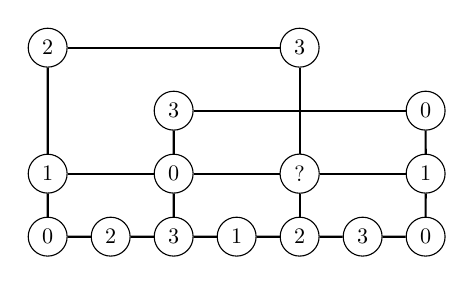
\begin{tikzpicture}[scale=0.8,every node/.style={transform shape}]
			\node[shape=circle,draw=black] (e) at (0,0) {?};
			\node[shape=circle,draw=black] (b) at (0,2) {3};
			\node[shape=circle,draw=black] (a-1) at (-2,0) {0};
			\node[shape=circle,draw=black] (a-2) at (-4,0) {1};
			\node[shape=circle,draw=black] (b-1) at (0,-1) {2};
			\node[shape=circle,draw=black] (a) at (2,0) {1};
			\node[shape=circle,draw=black] (ab) at (2,1) {0};
			\node[shape=circle,draw=black] (a-1b) at (-2,1) {3};
			\node[shape=circle,draw=black] (a-2b) at (-4,2) {2};
			\path[-, thick](ab) edge node[left] {} (a-1b);
			\path[-, thick](a) edge node[left] {} (ab);
			\path[-, thick](a-2b) edge node[left] {} (b);
			\path[-, thick](a-1) edge node[left] {} (a-1b);
			\path[-, thick](a-2) edge node[left] {} (a-2b);
			\path[-, thick](a-1) edge node[left] {} (a-2);
			\path[-, thick](a-1) edge node[left] {} (e);
			\path[-, thick](a) edge node[left] {} (e);
			\path[-, thick](b-1) edge node[left] {} (e);
			\path[-, thick](b) edge node[left] {} (e);
			
			
			\node[shape=circle,draw=black] (b-1a) at (1,-1) {3};
			\node[shape=circle,draw=black] (b-1a2) at (2,-1) {0};
			\node[shape=circle,draw=black] (b-1a-1) at (-1,-1) {1};
			\node[shape=circle,draw=black] (b-1a-2) at (-2,-1) {3};
			\node[shape=circle,draw=black] (b-1a-3) at (-3,-1) {2};
			\node[shape=circle,draw=black] (b-1a-4) at (-4,-1) {0};
			\path[-, thick](b-1) edge node[left] {} (b-1a);
			\path[-, thick](b-1a) edge node[left] {} (b-1a2);
			\path[-, thick](b-1) edge node[left] {} (b-1a-1);
			\path[-, thick](b-1a-1) edge node[left] {} (b-1a-2);
			\path[-, thick](b-1a-2) edge node[left] {} (b-1a-3);
			\path[-, thick](b-1a-3) edge node[left] {} (b-1a-4);
			\path[-, thick](a-2) edge node[left] {} (b-1a-4);
			\path[-, thick](a-1) edge node[left] {} (b-1a-2);
			\path[-, thick](a) edge node[left] {} (b-1a2);
			\end{tikzpicture}
		\end{figure}	
	\end{remark*}
	The previous example showed a locally admissible pattern that could not be extended to form a valid configuration of the group, and the main property of this example is that although the support of the chosen pattern can be taken to be a connected subgraph of the Cayley graph, it has a ``gap" which allows us to surround a position in such a way that the pattern could not be extended. A way of avoiding this type of pathological patterns is to require the supports of the patterns to have some sort of convexity.
	\begin{lemma} \label{lem.gcs_extend_to_rectangles} For every $n\ge 3$ any $n$-coloring of the rectangle $R_m$ can be extended to a proper $n$-coloring of the rectangle $R_{m+1}$.
	\end{lemma}
	\begin{proof}
		For every $k\in \{0,\ldots,m\}$ we define $$H_k\coloneqq \left(R_{m+1}\backslash R_{m}\right)\cap \{a^ib^k\mid i\ge 0\},$$
		which represents the elements of $R_{m+1}$ of height $k$, outside of the rectangle $R_m$. Note that by definition we have $$R_{m+1}=R_m\cup \bigcup_{k=0}^{m}H_k.$$ Then we can extend the pattern $p$ on $R_m$ by successive colorings (respecting the condition of being a proper coloring) coloring first $H_0$, then $H_1$, and so until we color $H_m$. In each step of this process each vertex has at most $2$ neighbors already colored, so having at least $3$ available colors is enough for this process to be carried out. 
	\end{proof}
	By using the same ideas present in the proof of the previous lemma we get the following proposition. Indeed, one can inductively color the rows of the Cayley graph one by one, so that each vertex has at most two colored neighbors at the moment it must choose its color. 
	\begin{proposition}\label{prop.gcs_rectangle_extension} For $n\ge 3$ every locally admissible pattern for $\mathcal{C}_n$ with support a rectangle is globally admissible.
	\end{proposition}
Now we can proceed to give estimates for the entropy of the GCS.
\begin{theorem} For $n\ge 3$, we have the following estimate for the topological entropy of the GCS $\mathcal{C}_n$:
	$$
	\log(n-2)\le \htop(\mathcal{C}_n)\le \log(n-1).
	$$
\end{theorem}
\begin{proof}
	Let us see that $\htop(\mathcal{C}_n)\le \log(n-1)$: a coloring of the rectangle $R_m$ may be extended to a coloring of the rectangle $R_{m+1}$ by coloring the remaining vertices having on each one at most $n-1$ options. With this
	\begin{align*}
	|\mathcal{L}_{R_{m+1}}(\mathcal{C}_n)|\le |\mathcal{L}_{R_m}(\mathcal{C}_{n})|(n-1)^{|R_{m+1}\backslash R_m|}.
	\end{align*}
	A simple calculation shows that $|R_{m+1}\backslash R_{m}|=N^m(mN+N-m)$. 
%	In effect, it suffices to notice that
%	\begin{align*}
%	R_{m+1}\backslash R_{m}&=\left\{a^ib^j\mid 0\le i<N^{m+1},\ 0\le k <m+1  \right\}\backslash \left\{a^ib^j\mid 0\le i<N^{m},\ 0\le k <m  \right\}\\
%	&=\left\{a^ib^j\mid N^m\le i<N^{m+1},\ 0\le k <m  \right\}\cup \left\{a^ib^m\mid 0\le i<N^{m+1} \right\},
%	\end{align*}
%	and that this union is disjoint. 
	With this:
	\begin{align*}
	\frac{1}{|R_{m+1}|}\log|\mathcal{L}_{R_{m+1}}(\mathcal{C}_n)|&=\frac{1}{(m+1)N^{m+1}}\log|\mathcal{L}_{R_{m+1}}(\mathcal{C}_n)|\\
	&\le \frac{1}{(m+1)N^{m+1}}\log|\mathcal{L}_{R_m}(\mathcal{C}_{n})|+\frac{N^m(mN+N-m)}{(m+1)N^{m+1}}\log(n-1)\\
	&=\frac{1}{N}\frac{m}{m+1}\frac{1}{mN^{m}}\log|\mathcal{L}_{R_m}(\mathcal{C}_{n})|+ \frac{mN+N-m}{m+1}\frac{1}{N}\log(n-1)\\
	&=\frac{1}{N}\frac{m}{m+1}\frac{1}{|R_m|}\log|\mathcal{L}_{R_m}(\mathcal{C}_{n})|+ \frac{m(N-1)+N}{m+1}\frac{1}{N}\log(n-1).
	\end{align*}
	Taking the limit $m\to \infty$ we arrive at
	\begin{align*}
	\htop(\mathcal{C}_n)&=\lim_{m\to \infty }	\frac{1}{|R_{m+1}|}\log|\mathcal{L}_{R_{m+1}}(\mathcal{C}_n)|\\
	&\le \lim_{m\to \infty }\frac{1}{N}\frac{m}{m+1}\frac{1}{|R_m|}\log|\mathcal{L}_{R_m}(\mathcal{C}_{n})| +\lim_{m\to \infty }\frac{m(N-1)+N}{m+1}\frac{1}{N}\log(n-1)\\
	&= \frac{1}{N}\htop(\mathcal{C}_n)+\frac{N-1}{N}\log(n-1),
	\end{align*}
	from where 
	 $$\htop(\mathcal{C}_n)\le \log(n-1).$$
	
	
	Now let us see that $\htop(\mathcal{C}_n)\ge \log(n-2)$:
	the rectangle $R_m$ can be colored starting from the upper levels to the lower levels, ensuring at least $n-2$ color options at each element, since in this way each vertex of the Cayley graph has at most two neighbors already colored. Then this coloring can be extended to the whole graph by using Proposition \ref{prop:gcs_rectnagleextension} and hence forming a globally admissible configuration for $\mathcal{C}_n$. From this we get that
	\begin{align*}
	|\mathcal{L}_{R_m}(\mathcal{C}_{n})|\ge (n-2)^{|R_m|},
	\end{align*}
	and so $\htop(\mathcal{C}_n)\ge \log(n-2)$.
\end{proof}
In particular, the lower bound from the previous proposition shows us that $\htop(\mathcal{C}_n)>0$ for every $n\ge 4$, but gives us no new information for the case of three colors $\mathcal{C}_3$, since by definition $\htop(\mathcal{C}_3)\ge 0$. In the next proposition we answer this question affirmatively, dividing the proof in two cases depending on the parity of $N$. If $N$ is odd we can exploit the fact that the Cayley graph of $\BS$ is bipartite (we know this since we have already constructed a $2$-coloring of it in Proposition \ref{prop.GCS_nonemptiness}, or equivalently observing that it has no odd cycles) to give a straightforward proof that the topological entropy of $\mathcal{C}_3$ is positive, while in the case of even $N$ we give a more delicate construction to arrive at the same result.
\begin{proposition} The GCS $\mathcal{C}_3\subseteq \{0,1,2\}^{\BS}$ has positive topological entropy.
\end{proposition}
\begin{proof}
	Let us start with the case of odd $N$. Here the Cayley graph of $\BS$ is bipartite and hence so is every rectangle $R_m$, for $m\ge 1$. Consider a \textit{partition} of $R_m$ into two sets $A$ and $B$, meaning that all edges of the graph are composed of a vertex in $A$ and a vertex in $B$. Then one of them, which we take to be $A$ without loss of generality, must have cardinality at least $\frac{1}{2}|R_m|$. Then we can create proper colorings of $R_m$ by coloring the vertices of $B$ with one color and have the freedom to choose between two colors for every vertex of $A$, and then extend this pattern on $R_m$ to the rest of the group as was said earlier.
	
	With the above we can estimate a lower bound for the number of proper colorings of $R_m$ by
	$$
	|\mathcal{L}_{R_m}(\mathcal{C}_3)|\ge 2^{|A|}\ge 2^{\frac{1}{2}|R_m|}.
	$$
	Then taking logarithm and dividing by $|R_m|$ we arrive at
	$$
	\frac{1}{|R_m|}\log |\mathcal{L}_{R_m}(\mathcal{C}_3)| \ge \frac{1}{2}\log (2),
	$$
	to finally take limit as $m\to \infty$ and obtain
	$$
	\htop(\mathcal{C}_3)\ge \frac{1}{2}\log(2)>0,
	$$
	which is what we wanted.
	
	
	Now consider the case of even $N$. For $m\ge 1$ we define a pattern $p\in \mathcal{A}^{R_{2m}}$, where some of the vertices of this rectangle will have the freedom of being assigned the symbol $1$ or $2$, in either case remaining a proper $3$-coloring of $R_{2m}$.
	
	First let us define 
	$$
	p|_{[e_{\BS},a^{N^{2m}-1}]}=\left(0(12)^{2N}\right)^{\infty}|_{[0,N^{2m}-1]},
	$$
and for $i\in \{0,\ldots, N^{2m}-1 \}$, $j\in \{0,\ldots, m-1 \}$ define
$$
p_{a^{i}b^{2j}}=p_{a^i}.
$$
That is, the symbols we see in the $a$-rows at even level of $R_{2m}$ are copies of the sequence found in the base of the rectangle. Now we proceed to define the pattern $p$ at the $a$-rows of odd level. Define for $i\in \left\{0,\ldots, \left\lfloor \frac{N^{2m}}{2N+1}\right\rfloor-1  \right\}$, $k\in \{0,\ldots,2N\}$, $j\in \{0,\ldots,m-1\}$ and any choice of $\alpha_{i,j,k}\in \{0,1\}$:
\begin{equation*}
p_{a^{(2N+1)i+k}b^{2j+1}}=\left\{
\begin{aligned}
 &\alpha_{i,j,k} \text{ if }k=0,\\
 & 0\text{ if }k=N \text{ or }k=N+1,\\
 & 2\text{ if }k\text{ is even and }k\neq N,\\
 & 1\text{ if }k\text{ is odd and }k\neq N+1.\\
\end{aligned}
\right.
\end{equation*}
With the above we are assigning to each $a$-row at odd level of $R_m$ (a subword of) the sequence $\left(\alpha_{i,j,k}\ 0\ (12)^{2N-2}\right)^{\infty}$, where every choice of $\alpha(i,j,k)\in \{1,2\}$ gives rise to a different pattern.

%	\begin{figure}[H]
%	\centering
%	\begin{tikzpicture}[scale=0.6,every node/.style={transform shape}]
%	\node[font=\Large] at (8,3) {$\vdots$};
%	\node[font=\Large] at (4,-1) {$\vdots$};
%	\node[font=\Large] at (12,-1) {$\vdots$};
%	\node[font=\Large] at (-1,1) {$\cdots$};
%	\node[font=\Large] at (17.5,1) {$\cdots$};
%	\node[shape=circle,draw=black] (a0) at (0,0) {0};
%	\node[shape=circle,draw=black] (a1) at (1,0) {1};
%	\node[shape=circle,draw=black] (a2) at (2,0) {2};
%	\node[shape=circle,draw=black] (a3) at (3,0) {1};
%	\node[shape=circle,draw=black] (a4) at (4,0)  {2};
%	\node[shape=circle,draw=black] (a5) at (5,0) {0};
%	\node[shape=circle,draw=black] (a6) at (6,0) {1};
%	\node[shape=circle,draw=black] (a7) at (7,0) {2};
%	\node[shape=circle,draw=black] (a8) at (8,0) {1};
%	\node[shape=circle,draw=black] (a9) at (9,0) {2};
%	\node[shape=circle,draw=black] (a10) at (10,0) {0};
%	\node[shape=circle,draw=black] (a11) at (11,0) {1};
%	\node[shape=circle,draw=black] (a12) at (12,0) {2};
%	\node[shape=circle,draw=black] (a13) at (13,0) {1};
%	\node[shape=circle,draw=black] (a14) at (14,0) {2};
%	\node[shape=circle,draw=black] (a15) at (15,0) {0};
%	\node[shape=circle,draw=black] (a16) at (16,0) {1};
%	\path[-, thick](e) edge node[left] {} (a1);
%	\foreach \x[remember=\x as \lastx (initially 0),evaluate=\x as \xx using int(\x)] in {1,...,16}
%	{
%		\path[-, thick](a\lastx) edge node[left] {} (a\x);
%	}
%	\node[shape=circle,draw=black] (b) at (0,1) {$\alpha$};
%	\node[shape=circle,draw=black] (a2b) at (2,1) {0};
%	\node[shape=circle,draw=black] (a4b) at (4,1) {2};
%	\node[shape=circle,draw=black] (a6b) at (6,1) {1};
%	\node[shape=circle,draw=black] (a8b) at (8,1) {0};
%	\node[shape=circle,draw=black] (a10b) at (10,1) {$\alpha $};
%	\node[shape=circle,draw=black] (a12b) at (12,1) {0};
%	\node[shape=circle,draw=black] (a14b) at (14,1) {2};
%	\node[shape=circle,draw=black] (a16b) at (16,1) {1};
%	\path[-, thick](e) edge node[left] {} (b);
%	\path[-, thick](a2) edge node[left] {} (a2b);
%	\path[-, thick](a4) edge node[left] {} (a4b);
%	\path[-, thick](a6) edge node[left] {} (a6b);
%	\path[-, thick](a8) edge node[left] {} (a8b);
%	\path[-, thick](a10) edge node[left] {} (a10b);
%	\path[-, thick](a12) edge node[left] {} (a12b);
%	\path[-, thick](a14) edge node[left] {} (a14b);
%	\path[-, thick](a16) edge node[left] {} (a16b);
%	\path[-, thick](b) edge node[left] {} (a2b);
%	\path[-, thick](a2b) edge node[left] {} (a4b);
%	\path[-, thick](a4b) edge node[left] {} (a6b);
%	\path[-, thick](a6b) edge node[left] {} (a8b);
%	\path[-, thick](a8b) edge node[left] {} (a10b);
%	\path[-, thick](a10b) edge node[left] {} (a12b);
%	\path[-, thick](a12b) edge node[left] {} (a14b);
%	\path[-, thick](a14b) edge node[left] {} (a16b);
%	\node[shape=circle,draw=black] (b2) at (0,2) {0};
%	\node[shape=circle,draw=black] (a4b2) at (4,2) {2};		
%	\node[shape=circle,draw=black] (a8b2) at (8,2) {1};
%	\node[shape=circle,draw=black] (a12b2) at (12,2) {2};
%	\node[shape=circle,draw=black] (a16b2) at (16,2) {1};
%	\path[-, thick](b) edge node[left] {} (b2);
%	\path[-, thick](a4b) edge node[left] {} (a4b2);
%	\path[-, thick](a8b) edge node[left] {} (a8b2);
%	\path[-, thick](a12b) edge node[left] {} (a12b2);
%	\path[-, thick](a16b) edge node[left] {} (a16b2);
%	\path[-, thick](b2) edge node[left] {} (a4b2);
%	\path[-, thick](a4b2) edge node[left] {} (a8b2);
%	\path[-, thick](a8b2) edge node[left] {} (a12b2);
%	\path[-, thick](a12b2) edge node[left] {} (a16b2);
%	\end{tikzpicture}
%\end{figure}



The above shows that
$$
|\mathcal{L}_{R_{2m}}(\mathcal{C}_3)|\ge 2^{m\left\lfloor \frac{N^{2m}}{2N+1}\right\rfloor },
$$
and hence
\begin{align*}
\frac{1}{|R_{2m}|}\log |\mathcal{L}_{R_{2m}}(\mathcal{C}_3)|&\ge\frac{m\left\lfloor \frac{N^{2m}}{2N+1}\right\rfloor}{2mN^{2m}}\log(2) \\
&\ge \frac{\frac{N^{2m}}{2N+1}-1}{2N^{2m}}\log(2).
\end{align*}
Finally, taking limit as $m\to\infty$ we obtain
$$
\htop(\mathcal{C}_3)\ge \frac{1}{2(2N+1)}\log(2)>0.
$$
\end{proof}
	
	\subsection{Mixing and frozen colorings}\label{subsection.mixing_and frozen}
Thanks to Proposition \ref{prop.loc_adm_5_colors} we know that for $n\ge 5$ we can extend any admissible pattern to a proper coloring of the Cayley graph of $\BS$, from which we obtain the following mixing property for $\mathcal{C}_n$.
\begin{theorem}\label{thm:gcs_mixing_n5} Let $n\ge 5$ and consider finite subsets $F_1,F_2\subseteq \BS$ such that 
	$$\left( F_1\cdot \{e_{\BS},a,a^{-1},a,b^{-1}\}\right)\cap F_2=\emptyset.$$
  Then for every choice of (locally) admissible patterns $p_i\in \{0,\ldots,n-1\}^{F_i}, i=1,2,$ there exists $x\in \mathcal{C}_n$ such that $x|_{F_1}=p_1$ and $x|_{F_2}=p_2$. With this we have that for $n\ge 5$ the GCS $\mathcal{C}_n$ is strongly irreducible.
\end{theorem}
\begin{proof}
	The above condition on $F_1$ and $F_2$ means that these two sets are disjoint, and separated by at least one vertex in the Cayley graph of $\BS$. 
	
	Consider two locally admissible patterns $p_i\in \{0,\ldots,n-1\}^{F_i}, i=1,2$. Then we can define a new pattern $p\in \{0,\ldots,n-1\}^{F_1\cup F_2}$ such that $p(f)=p_i(f)$ for $f\in F_i, i=1,2$ consistently, since $F_1\cap F_2=\emptyset.$ This pattern is also locally admissible thanks to the distance existing between $F_1$ and $F_2$, as between every vertex of $F_1$ and every vertex of $F_2$ there is at least one uncolored vertex. Then, according to Proposition \ref{prop.loc_adm_5_colors}, this pattern is globally admissible and hence there exists $x\in \mathcal{C}_n$ such that $x|_{F_1\cup F_2}=p$. This $x$ satisfies $x|_{F_1}=p_1$ and $x|_{F_2}=p_2$ and so we have found the desired point.
\end{proof}


The previous proposition tells us that for $n\ge 5$ the subshift $\mathcal{C}_n$ has a strong mixing property. On the other side, we can see that $\mathcal{C}_2$ has no type of mixing behavior: this $\BS$-subshift is either empty if $N$ is even, or if $N$ is odd then there is no way to assign the same color to two elements of the group $g,h\in \BS$ such that $g^{-1}h\in \left\{a^{2m+1}\mid m\in \mathbb{Z} \right\}$, which forbids the gluing of patterns at arbitrarily large distances. This contrast between $\mathcal{C}_2$ and $\mathcal{C}_n$ for $n\ge 5$ raises the question of what kind of mixing behaviors does $\mathcal{C}_3$ and $\mathcal{C}_4$ have. To study this we will use a similar approach as that of \cite{alon2019mixing}, by introducing the concept of a frozen coloring.
\begin{definition} Let $n\ge 3$. A configuration $x\in \mathcal{C}_n$ is called a \textbf{frozen coloring} if for every $y\in \mathcal{C}_n$ such that there exists a non-empty finite subset $F\subseteq \BS$ with $x|_{F^c}=y|_{F^c}$, then $x= y$. That is, no coloring of $\BS$ other than $x$ can coincide with it outside of any finite set.
\end{definition}

Frozen colorings are configurations in which the neighboring vertices of every finite subset of the Cayley graph determine unequivocally how this subset must be colored, in order to obtain a proper coloring. This behavior is the reason frozen colorings are closely related to the (lack of) mixing properties of the GCS, as the next proposition shows.
\begin{proposition} \label{prop:froz_col_not_si} If $\mathcal{C}_n$ has a frozen coloring, then it is not strongly irreducible.
\end{proposition}
\begin{proof}
	
	Looking for a contradiction, suppose that $\mathcal{C}_n$ is strongly irreducible and $x\in \mathcal{C}_n$ is a frozen coloring. 
	
	Consider any other configuration $y\in \mathcal{C}_n$ such that $y_{e_G}\neq x_{e_G}$. As $\mathcal{C}_n$ is strongly irreducible, there exists $F\subseteq G$ finite such that for any two patterns $p,q\in \mathcal{L}(\mathcal{C}_n)$ with $\mathrm{supp}(p)\cap \mathrm{supp}(q)\cdot F=\emptyset$ we have $[p]\cap [q]\neq \emptyset$. Considering the patterns $y|_{e_G}$ and $x|_{\partial B_M}$, where $\partial B_M\coloneqq \{g\in \BS: |g|=M\}$, for $M$ sufficiently large we have $\partial B_M \cap F= \emptyset$. Then there must exist a coloring $z\in \mathcal{C}_n$ such that $z_{e_G}=y_{e_G}\neq x_{e_G}$, and $z|_{\partial B_M}=x|_{\partial B_M}$. Moreover, we can assume that $z|_{B_{M-1}^c}=x|_{B_{M-1}^c}$, where $B_{M-1}\coloneqq \{g\in \BS: |g|\le M-1 \}$, since $z$ and $x$ coincide on $\partial B_M$ and hence re-coloring $z$ as $x$ outside of this ball gives us a proper coloring. 
	
	With this we have found a configuration $z\in \mathcal{C}_n$ which coincides with $x$ outside of a finite set but is different from $x$ inside it, so we have a contradiction with the fact that $x$ is a frozen coloring. Hence we conclude that any strongly irreducible subshift $\mathcal{C}_n$ cannot have a frozen coloring.
\end{proof}
We already know by Theorem \ref{thm:gcs_mixing_n5} that the GCS $\mathcal{C}_n$ for $n\ge 5$ is strongly irreducible, and hence by the above proposition it cannot have a frozen coloring. On the other hand, as the case $n=3$ is the first non-finite subshift of the GCS's $\mathcal{C}_n$ for any $N\ge 2$, it is reasonable to conjecture that its properties must still be somewhat rigid. The next proposition confirms this by showing that $\mathcal{C}_3$ possesses a frozen coloring, and with it exhibits the lack of a strong mixing behavior of the GCS with three colors.
\begin{theorem} The GCS $\mathcal{C}_3\subseteq \{0,1,2\}^{\BS}$ admits a frozen coloring, and hence is not strongly irreducible.
\end{theorem}
\begin{proof}The proof will be divided in three cases, depending on the value of $N \ (\mathrm{mod} \ 3)$. For each one of these cases we will construct explicitly the claimed frozen coloring.
	
	Let us suppose first that $N=1 \ (\mathrm{mod} \ 3)$, and with it for every $i\ge 0$ we have $N^i=1 \ (\mathrm{mod} \ 3)$.
	Let us define the configuration $x\in \{0,1,2\}^{\BS}$ such that for $g=b^{-j}a^k b^i\in \BS$ written in its normal form:
	$$
	x_g\coloneqq 2(i-j)+k \ (\mathrm{mod} \ 3).
	$$
	
	\begin{figure}[H]
		\centering
		\begin{tikzpicture}[scale=0.6,every node/.style={transform shape}]
		\node[font=\Large] at (8,3) {$\vdots$};
		\node[font=\Large] at (4,-1) {$\vdots$};
		\node[font=\Large] at (12,-1) {$\vdots$};
		\node[font=\Large] at (-1,1) {$\cdots$};
		\node[font=\Large] at (17.5,1) {$\cdots$};
		\node[shape=circle,draw=black] (a0) at (0,0) {0};
		\node[shape=circle,draw=black] (a1) at (1,0) {1};
		\node[shape=circle,draw=black] (a2) at (2,0) {2};
		\node[shape=circle,draw=black] (a3) at (3,0) {0};
		\node[shape=circle,draw=black] (a4) at (4,0)  {1};
		\node[shape=circle,draw=black] (a5) at (5,0) {2};
		\node[shape=circle,draw=black] (a6) at (6,0) {0};
		\node[shape=circle,draw=black] (a7) at (7,0) {1};
		\node[shape=circle,draw=black] (a8) at (8,0) {2};
		\node[shape=circle,draw=black] (a9) at (9,0) {0};
		\node[shape=circle,draw=black] (a10) at (10,0) {1};
		\node[shape=circle,draw=black] (a11) at (11,0) {2};
		\node[shape=circle,draw=black] (a12) at (12,0) {0};
		\node[shape=circle,draw=black] (a13) at (13,0) {1};
		\node[shape=circle,draw=black] (a14) at (14,0) {2};
		\node[shape=circle,draw=black] (a15) at (15,0) {0};
		\node[shape=circle,draw=black] (a16) at (16,0) {1};
		\path[-, thick](e) edge node[left] {} (a1);
		\foreach \x[remember=\x as \lastx (initially 0),evaluate=\x as \xx using int(\x)] in {1,...,16}
		{
			\path[-, thick](a\lastx) edge node[left] {} (a\x);
		}
		\node[shape=circle,draw=black] (b) at (0,1) {2};
		\node[shape=circle,draw=black] (a4b) at (4,1) {0};
		\node[shape=circle,draw=black] (a8b) at (8,1) {1};
		\node[shape=circle,draw=black] (a12b) at (12,1) {2};
		\node[shape=circle,draw=black] (a16b) at (16,1) {0};
		\path[-, thick](e) edge node[left] {} (b);
		\path[-, thick](a4) edge node[left] {} (a4b);
		\path[-, thick](a8) edge node[left] {} (a8b);
		\path[-, thick](a12) edge node[left] {} (a12b);
		\path[-, thick](a16) edge node[left] {} (a16b);
		\path[-, thick](b) edge node[left] {} (a4b);
		\path[-, thick](a4b) edge node[left] {} (a8b);
		\path[-, thick](a8b) edge node[left] {} (a12b);
		\path[-, thick](a12b) edge node[left] {} (a16b);
		\node[shape=circle,draw=black] (b2) at (0,2) {1};
		\node[shape=circle,draw=black] (a16b2) at (16,2) {2};
		\path[-, thick](b) edge node[left] {} (b2);
		\path[-, thick](a16b) edge node[left] {} (a16b2);
		\path[-, thick](b2) edge node[left] {} (a16b2);
		\end{tikzpicture}
	\end{figure}	
	
	Note that $gb=b^{-j}a^k b^{i+1}$ and $ga=b^{-j}a^k b^ia=b^{-j}a^{k+N^i}b^i$. With this, remembering that $N^i =1 \ (\mathrm{mod} \ 3)$ we have
	\begin{align*}
	x_{gb}&=x_g+2 \ (\mathrm{mod} \ 3), \text{ and} \\
	x_{ga}&=x_g+N^i \ (\mathrm{mod} \ 3) =x_g+1 \ (\mathrm{mod} \ 3).
	\end{align*}
	Therefore $x_{gb}\neq x_g$ and $x_{ga}\neq x_g$, and so $x\in \mathcal{C}_3$ defines a proper coloring. Let us see that $x$ defines a frozen coloring: looking for a contradiction let us suppose $y\in \mathcal{C}_3$ is such that there exists a finite subset $F\subseteq \BS$ with $y|_{F^ c}=x|_{F^c}$ and for every $f\in F: \ x_f\neq y_f$. By using the fact that $F$ is finite, and shifting both configurations if necessary, we may assume that $$F\subseteq \{g\in \BS\mid g=a^kb^i, \text{ for some }k\in \mathbb{Z}, i\ge 0\}.$$ 
	Geometrically, this means that $g$ is in the ``upper" section of the Cayley graph of $\BS$, that is, in a sheet having as a base the subgroup $\langle a\rangle$. Now consider $g$ in $F$ which maximizes the value of $i+k$ in its normal form. In other words,
	$$
	g\coloneqq \mathrm{argmax}\{i+k\mid g=a^kb^i\in F, \ k\in \mathbb{Z}, i\ge 0 \}.
	$$
	Then $y_{gb}=x_{gb}=x_g+2\ (\mathrm{mod} \ 3)$, and $y_{ga}=x_{ga}=x_g+1\ (\mathrm{mod} \ 3)$, and so as $y$ defines a proper coloring we must have $y_g=x_g$, but this gives a contradiction since as $g\in F$ we should have $y_g\neq x_g$.
	
	
	Now let us see the case $N=2\ (\mathrm{mod} \ 3)$. Note that now we have that for $i\ge 0$:
	\begin{equation*}	
	N^i=\left\{ 
	\begin{aligned}
	&1 \ (\mathrm{mod} \ 3) \text{ if }i\text{ is even}, \\
	&2 \ (\mathrm{mod} \ 3) \text{ if }i\text{ is odd.} 
	\end{aligned}
	\right.
	\end{equation*}
	Define a configuration  $x\in \{0,1,2\}^{\BS}$ such that for $g=b^{-j}a^k b^i\in \BS$ written in its normal form:
	$$
	x_g\coloneqq i-j+k \ (\mathrm{mod} \ 3).
	$$
	
	
	\begin{figure}[H]
		\centering
		\begin{tikzpicture}[scale=0.6,every node/.style={transform shape}]
		\node[font=\Large] at (8,3) {$\vdots$};
		\node[font=\Large] at (4,-1) {$\vdots$};
		\node[font=\Large] at (12,-1) {$\vdots$};
		\node[font=\Large] at (-1,1) {$\cdots$};
		\node[font=\Large] at (17.5,1) {$\cdots$};
		\node[shape=circle,draw=black] (a0) at (0,0) {0};
		\node[shape=circle,draw=black] (a1) at (1,0) {1};
		\node[shape=circle,draw=black] (a2) at (2,0) {2};
		\node[shape=circle,draw=black] (a3) at (3,0) {0};
		\node[shape=circle,draw=black] (a4) at (4,0)  {1};
		\node[shape=circle,draw=black] (a5) at (5,0) {2};
		\node[shape=circle,draw=black] (a6) at (6,0) {0};
		\node[shape=circle,draw=black] (a7) at (7,0) {1};
		\node[shape=circle,draw=black] (a8) at (8,0) {2};
		\node[shape=circle,draw=black] (a9) at (9,0) {0};
		\node[shape=circle,draw=black] (a10) at (10,0) {1};
		\node[shape=circle,draw=black] (a11) at (11,0) {2};
		\node[shape=circle,draw=black] (a12) at (12,0) {0};
		\node[shape=circle,draw=black] (a13) at (13,0) {1};
		\node[shape=circle,draw=black] (a14) at (14,0) {2};
		\node[shape=circle,draw=black] (a15) at (15,0) {0};
		\node[shape=circle,draw=black] (a16) at (16,0) {1};
		\path[-, thick](e) edge node[left] {} (a1);
		\foreach \x[remember=\x as \lastx (initially 0),evaluate=\x as \xx using int(\x)] in {1,...,16}
		{
			\path[-, thick](a\lastx) edge node[left] {} (a\x);
		}
		\node[shape=circle,draw=black] (b) at (0,1) {1};
		\node[shape=circle,draw=black] (a2b) at (2,1) {0};
		\node[shape=circle,draw=black] (a4b) at (4,1) {2};
		\node[shape=circle,draw=black] (a6b) at (6,1) {1};
		\node[shape=circle,draw=black] (a8b) at (8,1) {0};
		\node[shape=circle,draw=black] (a10b) at (10,1) {2};
		\node[shape=circle,draw=black] (a12b) at (12,1) {1};
		\node[shape=circle,draw=black] (a14b) at (14,1) {0};
		\node[shape=circle,draw=black] (a16b) at (16,1) {2};
		\path[-, thick](e) edge node[left] {} (b);
		\path[-, thick](a2) edge node[left] {} (a2b);
		\path[-, thick](a4) edge node[left] {} (a4b);
		\path[-, thick](a6) edge node[left] {} (a6b);
		\path[-, thick](a8) edge node[left] {} (a8b);
		\path[-, thick](a10) edge node[left] {} (a10b);
		\path[-, thick](a12) edge node[left] {} (a12b);
		\path[-, thick](a14) edge node[left] {} (a14b);
		\path[-, thick](a16) edge node[left] {} (a16b);
		\path[-, thick](b) edge node[left] {} (a2b);
		\path[-, thick](a2b) edge node[left] {} (a4b);
		\path[-, thick](a4b) edge node[left] {} (a6b);
		\path[-, thick](a6b) edge node[left] {} (a8b);
		\path[-, thick](a8b) edge node[left] {} (a10b);
		\path[-, thick](a10b) edge node[left] {} (a12b);
		\path[-, thick](a12b) edge node[left] {} (a14b);
		\path[-, thick](a14b) edge node[left] {} (a16b);
		\node[shape=circle,draw=black] (b2) at (0,2) {2};
		\node[shape=circle,draw=black] (a4b2) at (4,2) {0};		
		\node[shape=circle,draw=black] (a8b2) at (8,2) {1};
		\node[shape=circle,draw=black] (a12b2) at (12,2) {2};
		\node[shape=circle,draw=black] (a16b2) at (16,2) {0};
		\path[-, thick](b) edge node[left] {} (b2);
		\path[-, thick](a4b) edge node[left] {} (a4b2);
		\path[-, thick](a8b) edge node[left] {} (a8b2);
		\path[-, thick](a12b) edge node[left] {} (a12b2);
		\path[-, thick](a16b) edge node[left] {} (a16b2);
		\path[-, thick](b2) edge node[left] {} (a4b2);
		\path[-, thick](a4b2) edge node[left] {} (a8b2);
		\path[-, thick](a8b2) edge node[left] {} (a12b2);
		\path[-, thick](a12b2) edge node[left] {} (a16b2);
		\end{tikzpicture}
	\end{figure}	
	
	Then as before we have
	\begin{align*}
	x_{gb}&=x_g+1 \ (\mathrm{mod} \ 3), \text{ and} \\
	x_{ga}&=x_g+N^i \ (\mathrm{mod} \ 3),
	\end{align*}
	and so $x_{gb}\neq x_g$ and $x_{ga}\neq x_g$ (since $N^i$ can be either $1$ or $2$). With this we have that $x\in \mathcal{C}_3$ defines a proper coloring, so it only remains to prove that $x$ defines a frozen coloring. Looking for a contradiction, suppose there exists $y\in \mathcal{C}_3$ and a finite set $F\subseteq \BS$ such that $x|_{F^c}=y|_{F^c}$ and for every $f\in F: x_f\neq y_f$. Again, by shifting both configurations if necessary, we may assume that $F\subseteq \{g\in \BS\mid g=a^kb^i, \text{ for some }k\in \mathbb{Z}, i\ge 0\}$. Define $i_{max}\coloneqq \max\{ i\ge 0\mid a^kb^i\in F, \text{ for some }k\in \mathbb{Z}\}$ and $B_{max}\coloneqq\{g=a^kb^i\in F\mid i=i_{max}\}$.
	
	If $i_{max}$ is even, let us take $g=a^kb^i\in B_{max}$ which minimizes the value of $k$. Then as $i_{max}$ is even we have $N^{i_{max}}=1$ and with it $y_{gb}=x_{gb}=x_g+1  \ (\mathrm{mod} \ 3)$, and $y_{ga^{-1}}=x_{ga^{-1}}=x_g-N^{i_{max}} = x_g+2  \ (\mathrm{mod} \ 3)$. But then we must have $y_g=x_g$ and this gives a contradiction since $g\in F$ and therefore $x_g\neq y_g$.
	
	Now if $i_{max}$ is odd, let us consider the element $g=a^kb^i\in B_{max}$ which maximizes the value of $k$. Then as $i_{max}$ is odd we have $N^{i_{max}}=2$ and with it $y_{gb}=x_{gb}=x_g+1  \ (\mathrm{mod} \ 3)$, and $y_{ga}=x_{ga}=x_g+N^{i_{max}} = x_g+2  \ (\mathrm{mod} \ 3)$. But then we must have $y_g=x_g$ and this gives a contradiction since $g\in F$ and therefore $x_g\neq y_g$, proving that $x$ defines a frozen coloring.
	
	
	Finally suppose that $N=0 \ (\mathrm{mod} \ 3)$. The method used on the previous two cases to find a frozen coloring on $\mathcal{C}_3$ was to construct a configuration using a function $f(j,k,i)$ of the coefficients of the normal form of every element of the group, which $\mod \ 3$ had period $3$ on the variable $k$. This cannot be done in the case $N\in 3\mathbb{Z }$ since here the configuration constructed would satisfy $x=\sigma_{a^3}(x)$ and hence $x=\sigma_{a^N}(x)$ (since $N\in 3\mathbb{Z}$). But then by Proposition $\ref{prop:monochrom_col_easycase}$ the coloring $x$ would have to have monochromatic rows appearing on it, which contradicts the fact that $x\in \mathcal{C}_3$ defines a proper coloring. Nonetheless, using a similar but different kind of function we can define a configuration $x\in \{0,1,2\}^{\BS}$ such that for $g=b^{-j}a^k b^i\in \BS$ written in its normal form:
	$$
	x_g\coloneqq (k \ (\mathrm{mod} \ 2)) + 2(i-j) \ (\mathrm{mod} \ 3).
	$$
	
	\begin{figure}[H]
		\centering
		\begin{tikzpicture}[scale=0.6,every node/.style={transform shape}]
		\node[font=\Large] at (9,3) {$\vdots$};
		\node[font=\Large] at (4,-1) {$\vdots$};
		\node[font=\Large] at (12,-1) {$\vdots$};
		\node[font=\Large] at (-1,1) {$\cdots$};
		\node[font=\Large] at (19.5,1) {$\cdots$};
		\node[shape=circle,draw=black] (e) at (0,0) {0};
		\node[shape=circle,draw=black] (a1) at (1,0) {1};
		\node[shape=circle,draw=black] (a2) at (2,0) {0};
		\node[shape=circle,draw=black] (a3) at (3,0) {1};
		\node[shape=circle,draw=black] (a4) at (4,0)  {0};
		\node[shape=circle,draw=black] (a5) at (5,0) {1};
		\node[shape=circle,draw=black] (a6) at (6,0) {0};
		\node[shape=circle,draw=black] (a7) at (7,0) {1};
		\node[shape=circle,draw=black] (a8) at (8,0) {0};
		\node[shape=circle,draw=black] (a9) at (9,0) {1};
		\node[shape=circle,draw=black] (a10) at (10,0) {0};
		\node[shape=circle,draw=black] (a11) at (11,0) {1};
		\node[shape=circle,draw=black] (a12) at (12,0) {0};
		\node[shape=circle,draw=black] (a13) at (13,0) {1};
		\node[shape=circle,draw=black] (a14) at (14,0) {0};
		\node[shape=circle,draw=black] (a15) at (15,0) {1};
		\node[shape=circle,draw=black] (a16) at (16,0) {0};
		\node[shape=circle,draw=black] (a17) at (17,0) {1};
		\node[shape=circle,draw=black] (a18) at (18,0) {0};
		\path[-, thick](e) edge node[left] {} (a1);
		\foreach \x[remember=\x as \lastx (initially 0),evaluate=\x as \xx using int(\x)] in {1,...,18}
		{
			\path[-, thick](a\lastx) edge node[left] {} (a\x);
		}
		\node[shape=circle,draw=black] (b) at (0,1) {2};
		\node[shape=circle,draw=black] (a3b) at (3,1) {0};
		\node[shape=circle,draw=black] (a6b) at (6,1) {2};
		\node[shape=circle,draw=black] (a9b) at (9,1) {0};
		\node[shape=circle,draw=black] (a12b) at (12,1) {2};
		\node[shape=circle,draw=black] (a15b) at (15,1) {0};
		\node[shape=circle,draw=black] (a18b) at (18,1) {2};
		\path[-, thick](e) edge node[left] {} (b);
		\path[-, thick](a3) edge node[left] {} (a3b);
		\path[-, thick](a6) edge node[left] {} (a6b);
		\path[-, thick](a9) edge node[left] {} (a9b);
		\path[-, thick](a12) edge node[left] {} (a12b);
		\path[-, thick](a15) edge node[left] {} (a15b);
		\path[-, thick](a18) edge node[left] {} (a18b);
		\path[-, thick](b) edge node[left] {} (a3b);
		\path[-, thick](a3b) edge node[left] {} (a6b);
		\path[-, thick](a6b) edge node[left] {} (a9b);
		\path[-, thick](a9b) edge node[left] {} (a12b);
		\path[-, thick](a12b) edge node[left] {} (a15b);
		\path[-, thick](a15b) edge node[left] {} (a18b);
		\node[shape=circle,draw=black] (b2) at (0,2) {1};
		\node[shape=circle,draw=black] (a9b2) at (9,2) {2};
		\node[shape=circle,draw=black] (a18b2) at (18,2) {1};
		\path[-, thick](b) edge node[left] {} (b2);
		\path[-, thick](a9b) edge node[left] {} (a9b2);
		\path[-, thick](a18b) edge node[left] {} (a18b2);
		\path[-, thick](b2) edge node[left] {} (a9b2);
		\path[-, thick](a9b2) edge node[left] {} (a18b2);
		\end{tikzpicture}
	\end{figure}
	
	
	
	We see that since $N^i$ is odd for every $i\ge 0$ we have:
	\begin{align*}
	x_{gb}&=x_g+2\ (\mathrm{mod} \ 3), \text{ and} \\
	x_{ga}&=(k+N^i \ (\mathrm{mod} \ 2)) + 2(i-j) \ (\mathrm{mod} \ 3)=x_g+1 \ (\mathrm{mod} \ 3),
	\end{align*}
	from which $x\in \mathcal{C}_3$ defines a proper coloring, and we can proceed as we did previously in the case $N^i=1\ (\mathrm{mod} \ 3)$. That is, to prove that $x$ defines a frozen coloring we suppose $y\in \mathcal{C}_3$ is such that there exists a finite subset $F\subseteq \BS$ with $y|_{F^ c}=x|_{F^c}$ and for every $f\in F: \ x_f\neq y_f$. By shifting both configurations if necessary, we may assume that $F\subseteq \{g\in \BS\mid g=a^kb^i, \text{ for some }k\in \mathbb{Z}, i\ge 0\}$. Now let us consider $g$ in $F$ which maximizes the value of $i+k$ in its normal form. Then $y_{gb}=x_{gb}=x_g+2\ (\mathrm{mod} \ 3)$, and $y_{ga}=x_{ga}=x_g+1\ (\mathrm{mod} \ 3)$, and so as $y$ defines a proper coloring we must have $y_g=x_g$, but this gives a contradiction since as $g\in F$ we should have $y_g\neq x_g$. Hence we see that $x$ a frozen coloring.
	
	To finish the proof we simply use the previous proposition to see that $\mathcal{C}_3$ cannot be strongly irreducible, as we have constructed a frozen coloring in it.
\end{proof}

This last theorem together with the previous comments settle the existence of frozen colorings for $n=3$ and $n\ge 5$. To tackle the case of four colors, and in the process give an alternative proof of the lack of frozen colorings for $n\ge 5$, we will use a proposition from \cite{alon2019mixing} used in that paper to prove the lack of frozen $q$-colorings in $\mathbb{Z}^d$ for $q\ge d+2$.

\begin{proposition}[\cite{alon2019mixing}]\label{prop:nofroz_graph} For a graph $\Gamma$ let us define its \textbf{edge-isoperimetric constant} by
	$$
	i_e(\Gamma)\coloneqq \inf_{F\subseteq \Gamma \text{ finite}}\frac{|E(F,\Gamma\backslash F)|}{|F|},
	$$
	where $E(F,\Gamma\backslash F)$ are the edges of $\Gamma$ connecting vertices from $F$ to $\Gamma\backslash F$. Denote by $\Delta$ the maximum degree of $\Gamma$. Then for every $q>\frac{1}{2}\Delta+\frac{1}{2}i_e(\Gamma)+1$ there do not exist frozen $q$-colorings of $\Gamma$.
\end{proposition}
%\begin{proof}
%	We denote $\Gamma=(V,E)$, and for $F\subseteq V$ we use the notation $E(F,F)$ for the edges of $E$ that connect vertices from $F$ with each other, and $E(F,\Gamma\backslash F)$ for the edges of $E$ that connect vertices from $F$ with vertices from the rest of the graph.
%	
%	Given a subset of vertices $F\subseteq V$ we say that a $q$-coloring $x$ of $\Gamma$ is frozen on $F$ if for every subset $F'\subseteq F$ and every $q$-coloring $y$ of $\Gamma$ such that $x|_{F'^c}=y|_{F'^c}$, then $x=y$. Hence $x$ is a frozen $q$-coloring if and only if $x$ is a frozen $q$-coloring of $F$, for every finite subset $F\subseteq V$. 
%	
%	We are going to prove the following claim: for every $F\subseteq V$ finite, if $$(q-1)|F|\ge |E(F,F)|+|E(F,\Gamma\backslash F)|,$$ then no $q$-coloring of $\Gamma$ is frozen on $F$. In particular, as $2|E(F,F)|+|E(F,\Gamma\backslash F)|$ equals the sum of the degrees of vertices in $F$, we conclude that if $(q-1-\frac{\Delta}{2})|F|>\frac{1}{2}|E(F,\Gamma\backslash F)|$ then
%	$$
%	(q-1)|F|>\frac{\Delta}{2}|F|+\frac{1}{2}|E(F,\Gamma\backslash F)|\ge |E(F,F)|+|E(F,\Gamma\backslash F)|,
%	$$
%	and hence no $q$-coloring of $\Gamma$ is frozen of $F$. With this the proposition follows immediately, since if $q>\frac{1}{2}\Delta+\frac{1}{2}i_e(\Gamma)+1$ then there must exist some finite subset $F\subseteq V$ such that $$q>\frac{1}{2}\Delta+\frac{1}{2}\frac{|E(F,\Gamma\backslash F)|}{|F|}+1,$$
%	from which $(q-1-\frac{\Delta}{2})|F|>\frac{1}{2}|E(F,\Gamma\backslash F)|$ and so no $q$-coloring of $\Gamma$ is frozen on $F$, and in particular no $q$-coloring of $\Gamma$ can be a frozen coloring. 
%	
%	We now proceed to prove the claim. Suppose there exists a $q$-coloring $x$ which is frozen on $F$. Consider the subgraph $\Gamma'=(F\cup N(F),E(F)\cup E(F,\Gamma\backslash F))$ where $N(F)$ is the neighborhood of $F$ on $\Gamma$. For distinct colors $i,j$ denote by $\Gamma_{i,j}'$ the subgraph of $\Gamma'$ consisting of edges between vertices which $x$ colors with $i$ and $j$, and call the connected components of these subgraphs the bi-color components. Note that the family of bi-color components $\mathcal{A}$ partition the edges of $\Gamma'$, so we have $\sum_{A\in \mathcal{A}}|E(A)|=|E(F)|+|E(F,\Gamma\backslash F)|$. Note also that each $A\in \mathcal{A}$ must contain a vertex of $N(F)$ since otherwise we could interchange both colors appearing on the vertices of $A$ and obtain a valid coloring, contradicting the fact that $x$ is frozen on $F$. With this $|A\cap F|\le |E(A)|$. Note also that each vertex of $F$ has $q-1$ colors as neighbours, again since otherwise we could change the color of the vertex to obtain a new $q$-coloring and contradict that $x$ is frozen on $F$. With this we see that $\sum_{A\in \mathcal{A}}|A\cap F|=(q-1)|F|$, and so getting all this together:
%	$$
%	(q-1)|F|=\sum_{A\in \mathcal{A}}|A\cap F|\le \sum_{A\in \mathcal{A}}|E(A)|=|E(F)|+|E(F,\Gamma\backslash F)|,
%	$$
%	which contradicts the hypothesis of the claim.
%\end{proof}
\begin{theorem} For $n\ge 4$ the GCS $\mathcal{C}_n$ does not admit a frozen coloring.
\end{theorem}
\begin{proof}
	Denoting by $\Gamma$ the Cayley graph of $\BS$ its maximum degree is $\Delta=4$, and if we prove that $i_e(\Gamma)=0$ we will have that, using proposition \ref{prop:nofroz_graph}, for $q>\frac{1}{2}\cdot 4+\frac{1}{2}\cdot 0+1=3$ this graph does not admit frozen $q$-colorings, proving the statement.
	
	Let us see that $i_e(\Gamma)=0$. Consider for every $k\ge 1: \ \gamma_{k}\coloneqq E(R_k,\Gamma\backslash R_k)$. We see that $\gamma_1=2N+2$, and that for every $k\ge 2$:
	$$
	\gamma_k=N^k+2+N(\gamma_{k-1}-N^{k-1})=2+N\gamma_{k-1},
	$$
	by using the fact that the $N$ sheets arising from the base of the rectangle $R_k$ are copies of the rectangle $R_{k-1}$. 
	With this we have that 
	$$
	\gamma_{k+1}-\gamma_{k}=N(\gamma_k-\gamma_{k-1}), \ \gamma_{2}-\gamma_{1}=2N^2,
	$$
	and so $\gamma_{k}-\gamma_{k-1}=2N^k$, for every $k\ge 2$. Now summing this equality from $k=2$ to $k=m$ we see that
	\begin{align*}
	\gamma_{m}-(2N+2)=\gamma_{m}-\gamma_{1}=\sum_{k=2}^m \gamma_{k}-\gamma_{k-1}&=2\sum_{k=2}^m N^k \\
	&= 2\frac{N^{m+1}-N^2}{N-1},
	\end{align*}
	and hence $\gamma_{m}=2\frac{N^{m+1}-1}{N-1}$. From this calculation we can estimate the edge-isoperimetric constant:
	$$
	i_e(\Gamma)\le \liminf_{m\to \infty}\frac{|E(R_m,\Gamma\backslash R_m|)}{|R_m|}=\liminf_{m\to \infty}\frac{\gamma_m}{|R_m|}=\liminf_{m\to \infty}\frac{2}{mN^m}\frac{N^{m+1}-1}{N-1}=0,
	$$
	and so $i_e(\Gamma)=0$ as we had claimed at the beginning of the proof.
\end{proof}
	
	
	\newpage 
	
we still don't know if this kind of construction is always possible. To our knowledge the following question remains open:
	\begin{question*}
	dssad?
	\end{question*}
	
	
	\textbf{Acknowledgements}. I would like to thank my Master's advisor Michael Schraudner for his continuous support, and Nathalie Aubrun for her helpful comments and ideas. This work was developed as part of a Master's degree thesis, partially supported by CONICYT-PFCHA/Magíster Nacional/2019 - 22190176.
	
	%%%%%%%%%%%%%%%%%%%%%%%
	%%%%%%%%%%%%%%%%%%%%%%%
	\bibliographystyle{plain}
	\bibliography{bibliography}{}
\end{document}